% -*- TeX:SI -*- slovene sub-mode for spell check
%%%%%%%%%%%%%%%%%%%%%%%%%%%%%%%%%%%%%%%%%%%%%%%%%%%%%%%%%%%%%%%%%%%%%%%%%%%%%%%%%%%%%%%%%%%%%%%%%%%%%%%%%%%%%%%%%%%%%%%%
% LaTeX predloga za zaključna dela Univerza v Ljubljani, Fakulteta za elektrotehniko Zbral in uredil: Roman Kamnik, junij 2013 Dopolnil: Sebastjan Šlajpah (2013), Sašo Tomažič (2013), Peter Miklavčič
% (2019)
%%%%%%%%%%%%%%%%%%%%%%%%%%%%%%%%%%%%%%%%%%%%%%%%%%%%%%%%%%%%%%%%%%%%%%%%%%%%%%%%%%%%%%%%%%%%%%%%%%%%%%%%%%%%%%%%%%%%%%%%
\documentclass[a4paper,twoside,openright,12pt,slovene]{book}
\usepackage[pdftex]{UNI-LJ-FE-Diploma} % stil zaključnega dela UL FE
\usepackage[utf8]{inputenc} % predloga uporablja standardno kodiranje Unicode UTF-8, ki podpira šumnike
\usepackage[greek,english,slovene]{babel} % seznam uporabljenih jezikov (zadnji na seznamu je primarni)
\usepackage{svg}

% PDF/A %%%%%%%%%%%%%%%%%%%%%%%%%%%%%%%%%%%%%%%%%%%%%%%%%%%%%%%%%%%%%%%%%%%%%%%%%%%%%%%%%%%%%%%%%%%%%%%%%%%%%%%%%%%%%%%% Več o PDF/A v LaTeX-u: https://www.mathstat.dal.ca/~selinger/pdfa/
\usepackage{filecontents}
\begin{filecontents*}{\jobname.xmpdata}
    \Title{Vpeljava HFSI algoritma v brezsenzorski pogon} % Mora biti enak kot je v prijavi teme!
    \Author{Matic Gregorčič} % Mora biti enak kot na naslovnici!
\end{filecontents*}
\usepackage[a-1b]{pdfx}
%%%%%%%%%%%%%%%%%%%%%%%%%%%%%%%%%%%%%%%%%%%%%%%%%%%%%%%%%%%%%%%%%%%%%%%%%%%%%%%%%%%%%%%%%%%%%%%%%%%%%%%%%%%%%%%%%%%%%%%%

% LaTeX PAKETI %%%%%%%%%%%%%%%%%%%%%%%%%%%%%%%%%%%%%%%%%%%%%%%%%%%%%%%%%%%%%%%%%%%%%%%%%%%%%%%%%%%%%%%%%%%%%%%%%%%%%%%%% Kompakten pregled LaTeX ukazov je dostopen na
% https://en.wikibooks.org/wiki/Category:Book:LaTeX Navodila posameznih uporabljenih paketov so dostopna na https://www.ctan.org

% Dodatni simboli
\usepackage{textcomp}                               % dodatni simboli (kot npr. €)
\usepackage{gensymb}                                % dodatni simboli \de­gree, \cel­sius, \pert­hou­sand, \mi­cro, \ohm
\newcommand{\uppi}{\textrm{\greektext p\latintext}} % velika grška črka P z \uppi, alternativa simbolu \Pi

% Osnovno oblikovanje
\hypersetup{unicode,hidelinks,breaklinks,hyperindex} % dodatne možnosti hiperpovezav
\usepackage[normalem]{ulem}                          % podčrtavanje in prečrtavanje teksta
\usepackage{float}                                   % dodatne možnosti oblikovanja objektov
\usepackage{enumitem}                                % dodatne možnosti oblikovanja seznamov

% Dodatno oblikovanje \zamaknirobsodihstrani{0mm} % dodatna prilagoditev levega roba sodih strani za dvostranski tisk \usepackage{dcolumn}        % poravnava po decimalnih mestih v tabelah
%\usepackage{longtable}      % večstranske tabele \usepackage{caption}        % dodatne možnosti označevanja objektov \usepackage{rotating}       % vretenje objektov, strani, ipd.

% Matematična orodja
\usepackage{mathtools} % http://mirrors.ctan.org/macros/LaTeX/contrib/mathtools/mathtools.pdf
\usepackage{bm}        % ukaz za odebeljeni tisk \bm v matematičnih okoljih
%\usepackage{cancel}   % ukaz za prečrtavanje \cancel v matematičnih okoljih

% Grafična orodja
\usepackage{graphicx}                 % vključevanje bitnih slik z ukazom \includegraphics
\usepackage{grffile}                  % podpora presledkom pri ukazu \includegraphics
%\usepackage{tikz}                    % paket TikZ za risanje (npr. blokovnih shem, diagramov poteka, itd.) \usetikzlibrary{calc,shapes,arrows}  % dodatne možnosti paketa TikZ \usepackage{tikzscale}
%% skaliranje risb \usepackage[smartlabels]{circuitikz} % risanje shem vezij \usepackage{pgfplots}                % paket PGFPlots za risanje grafov, tudi iz CSV in podobnih datotek
%\usepgfplotslibrary{polar,external}  % dodatne možnosti paketa PGFPlots \usepackage{tikz-3dplot}             % 3D risanje Primeri: http://texample.net , http://pgfplots.net/tikz/examples ,
%http://pgfplots.sourceforge.net/gallery.html

% Vključevanje datotek
\usepackage{pdfpages} % vključevanje PDF datotek z ukazom \includegraphics
\usepackage{epstopdf} % vključevanje EPS datotek z ukazom \includegraphics
\usepackage{svg} % vključevanje EPS datotek z ukazom \includegraphics
\usepackage{listings} % orodja za izpisovanje programske kode
\lstset{              % nastavitve orodja za izpisovanje programske kode
    basicstyle=\ttfamily\footnotesize, breaklines=true, numbers=left, numberstyle=\scriptsize, keywordstyle=\color{blue}, commentstyle=\color{unilj}, stringstyle=\color{olive}, }
%%%%%%%%%%%%%%%%%%%%%%%%%%%%%%%%%%%%%%%%%%%%%%%%%%%%%%%%%%%%%%%%%%%%%%%%%%%%%%%%%%%%%%%%%%%%%%%%%%%%%%%%%%%%%%%%%%%%%%%%

% DEKLARACIJE %%%%%%%%%%%%%%%%%%%%%%%%%%%%%%%%%%%%%%%%%%%%%%%%%%%%%%%%%%%%%%%%%%%%%%%%%%%%%%%%%%%%%%%%%%%%%%%%%%%%%%%%%%
\naslov{Vpeljava HFSI algoritma v brezsenzorski pogon} % Mora biti enak kot je v prijavi teme!
\avtor{Matic Gregorčič} % Mora se ujemati s \Title pri metapodatkih PDF/A!
\mentor{Mitja Nemec}
%\somentor{Naziv, ime in priimek somentorja}
\date{Ljubljana, \the\year}
\univerza{Univerza v Ljubljani}
\definecolor{unilj}{cmyk}{0.00, 0.94, 0.94, 0.06} % barva Univerze v Ljubljani

% Potrebno je paziti, da je izbrana prava kombinacija tipa dela in sodelujočih fakultet glede na študijski program!
\delo{Magistrko delo\\~\\Univerzitetni študijski program druge stopnje Elektrotehnika}
%\delo{Diplomsko delo\\~\\Univerzitetni študijski program prve stopnje Multimedija} \delo{Diplomsko delo\\~\\Visokošolski strokovni študijski program\\prve stopnje Aplikativna elektrotehnika}
%\delo{Diplomsko delo\\~\\Visokošolski strokovni študijski program\\prve stopnje Multimedijske komunikacije} \delo{Magistrsko delo\\~\\Magistrski študijski program druge stopnje Elektrotehnika}
%\delo{Magistrsko delo\\~\\Magistrski študijski program druge stopnje Uporabna statistika}
\fakulteta{Fakulteta za elektrotehniko}
%\fakulteta{Fakulteta za elektrotehniko,\\Fakulteta za računalništvo in informatiko} % Za program Multimedija \fakulteta{Fakulteta za elektrotehniko, Biotehniška fakulteta,\\Ekonomska fakulteta,
%Fakulteta za družbene vede,\\Fakulteta za matematiko in fiziko, Fakulteta za\\računalništvo in informatiko, Medicinska fakulteta} % Za program Uporabna statistika
%%%%%%%%%%%%%%%%%%%%%%%%%%%%%%%%%%%%%%%%%%%%%%%%%%%%%%%%%%%%%%%%%%%%%%%%%%%%%%%%%%%%%%%%%%%%%%%%%%%%%%%%%%%%%%%%%%%%%%%%

% DOKUMENT %%%%%%%%%%%%%%%%%%%%%%%%%%%%%%%%%%%%%%%%%%%%%%%%%%%%%%%%%%%%%%%%%%%%%%%%%%%%%%%%%%%%%%%%%%%%%%%%%%%%%%%%%%%%%
\begin{document}
\frontmatter

\selectlanguage{slovene}

%******************************* NASLOVNICA ************************************
\maketitle

%******************************* ZAHVALA ***************************************
\zahvala

Iskrene zahvale mentorju doc. dr. Mitji Nemcu za vso pomoč in napotke, ki ste jih nudili skozi izvedbo tega dela. 

Hvala podjetju, ki je omogočilo izvedbo te naloge in vsem sodelavcem za ideje in spodbudo.

Zahvalil bi se tudi družini, ki mi je stala ob strani in me podpirala v času pisanja tega dela.

%******************************* POVZETEK IN KLJUČNE BESEDE ********************
\povzetek
HFSI algoritem z visokofrekvenčnim signalom vzbuja stator stroja, preko tokovnega odziva pa oceni pozicijo rotorja. S FOC vodenjem pa se nato vodi prečni tok, ki tvori navor. Prednost te metode
proti klasičnem zagonu motorja, kjer ustvarimo vrtirajoče magnetno polje, je robustnost zagona, maksimalni navor in manjša verjetnost desinhronizacije stroja. 

V prvem poglavju predstavimo stroj IPMSM, ki se je uporabljal pri izdelavi te metode in ga matematično opišemo. V naslednjem poglavju opišemo delovanje HFSI metode, izpeljemo pričakovani tokovni odziv
visokofrekvečnega vzbujanja in pokažemo odziv na realnem sistemu in kako ta odstopa od idealnega. Proti koncu poglavja predstavimo ocenjene pozicije iz tokovnih odzivov. 

V četrtem poglavju prikažemo implementacijo v celoten sistem in FOC vodenje stroja. V zadnjem poglavju pa predstavimo eksperimentalni sistem, na katerem je bil algoritem HFSI razvit, kako merimo tok
in krmilimo napetost ter pokažemo oceno pozicije pri različnih pogojih.

\kljucnebesede
Vzbujanje z visokofrekvenčnim signalom, izraženi poli, ocena pozicije rotorja pri nizkih hitrostih, IPMSM, FOC

\selectlanguage{english}

%******************************* ABSTRACT AND KEYWORDS *************************

\abstract


\keywords
High frequency signal injection, saliency, rotor position estimation at low speeds, IPMSM, FOC

\selectlanguage{slovene}

%******************************* KAZALO ****************************************
\tableofcontents

%******************************* SEZNAM SLIK, SEZNAM TABEL *********************
\seznamslik
%\seznamtabel

%******************************* SEZNAM SIMBOLOV *******************************
\seznamsimbolov
V pričujočem zaključnem delu so uporabljene naslednje veličine in simboli:

\begin{center}
    \begin{tabular}{*{4}{l}} \hline
        \multicolumn{2}{c}{\bf{Veličina / oznaka}}           & \multicolumn{2}{c}{\bf{Enota}} \\ \hline
        Ime                                                        & Simbol                                 & Ime                  & Simbol                 \\ \hline
        Vzbujanje z visokofrekvečnim signalom                      & HFSI                                   & -                    & -                      \\
        Rotorski koordinatni sistem                                & RKS                                    & -                    & -                      \\
        Statorski koordinatni sistem                               & SKS                                    & -                    & -                      \\
        Koordinatni sistem HFSI metode                             & HKS                                    & -                    & -                      \\
        FOC koordinatni sistem                                     & FKS                                    & -                    & -                      \\
        Regulacija z orientacijo polja                             & FOC                                    & -                    & -                      \\
        Sinhronski motor z vlitimi permanentnimi magneti           & IPMSM                                  & -                    & -                      \\
        Fazno zaklenjena zanka                                     & PLL                                    & -                    & -                      \\
        Visoka frekvenca                                           & VF                                     & -                    & -                      \\
        Prepustni pasovni filter                                   & BPF                                    & -                    & -                      \\
        Zaporni pasovni filter                                     & BSF                                    & -                    & -                      \\
        PI regulator                                               & PI                                     & -                    & -                      \\                                                    
        Koordinati SKS                                             & $\alpha$; $\beta$                      & -                    & -                      \\
        Koordinati RKS                                             & $d$; $q$                               & -                    & -                      \\
        Koordinati HKS                                             & $dh$; $qh$                             & -                    & -                      \\
        Koordinati FKS                                             & $df$; $qf$                             & -                    & -                      \\
        Električni kot rotorja                                     & $\theta_{r}$                           & radian               & rad                    \\
        Odklon FKS                                                 & $\theta_{f}$                           & radian               & rad                    \\
        Odklon HKS                                                 & $\theta_{h}$                           & radian               & rad                    \\
        Induktivnost v vzdolžni in prečni smeri                    & $L_d; L_q$                             & Henry                & H                      \\
        Statorska upornost                                         & $R_s$                                  & ohm                  & $\Omega$               \\
        Električna kotna hitrost rotorja                           & $\omega_r$                             & radian na sekundo    & $rad \cdot s^{-1}$     \\
        Frekvenca vzbujalnega signala                              & $\omega_{s}$                           & radian na sekundo    & $rad \cdot s^{-1}$     \\
        Število polov                                              & $p$                                    & -                    & -                      \\
        Napetost v vzdolžni in prečni smeri                        & $u_{d}; u_{q}$                         & volt                 & V                      \\
        Tok v vzdolžni in prečni smeri                             & $i_{d}; i_{q}$                         & ampere               & A                      \\
        VF napetostno vzbujanje                                    & $u^{VF}_{dh}; u^{VF}_{qh}$             & volt                 & V                      \\
        VF tokovni odziv                                           & $i^{VF}_{dh}; i^{VF}_{qh}$             & ampere               & A                      \\
        Amplituda VF napetostnega vzbujanja                        & $U_h$                                  & volt                 & V                      \\
        Amplituda VF tokovnega odziva                              & $I_{dh}; I_{qh}$                       & ampere               & A                      \\
        Napajalna napetost razsmernika                             & $U_{DC}$                               & volt                 & V                      \\
        Mrtvi čas                                                  & $t_m$                                  & sekunda              & s                      \\
    \end{tabular}
\end{center}

\mainmatter

%******************************* UVOD ******************************************
\chapter{Uvod} \label{uvod}

V industriji se opazi vedno večja uporaba brezkrtačnih sinhronih strojev, zaradi njihove specifične gostote moči in dobre učinkovitosti. Vendar pa za vodenje takih motorjev potrebujemo dražje in bolj
kompleksne pretvornike. Pri vodenju sinhronih strojev je kritično poznavanje pozicije rotorja. To merimo z dajalnikom pozicije, ki pa ima slabosti kot so povišana cena, dodatna mehanska komponenta, ki
se lahko pokvari, prav tako pa terja dodaten korak v proizvodnji takih strojev. 

Zato se za vodenje uporabijo brezsenzorski algoritmi, ki pozicijo rotorja ocenjujejo iz drugih merjenih veličin. Tem algoritmom pravimo opazovalniki in jih delimo na tiste, ki imajo delovno območje
pri višjih vrtilnih hitrostih in na opazovalnike, ki delujejo pri nižjih. Pri višjih hitrostih se to stori z angl. Sliding Mode Observer (SMO) opazovalnikom, ki ocenjuje inducirano napetost stroja, preko te pa pozicijo. Pri nižjih
hitrostih pa je inducirana napetost premajhna za uporabo takega opazovalnika. Zato se ponavadi uporablja metoda zagona motorja, kjer v statorju ustvarimo vrtirajoče magnetno polje, ki pospeši rotor do
željene hitrosti, nato pa se uporabi SMO opazovalnik. Tak zagon motorja lahko odpove pri višjih bremenskih navorih, zato se uporabljajo metode, ki izrabljajo pojav izraženih polov in preko tega pojava
ocenjujejo pozicijo rotorja. To magistrsko delo obravnava eno od takih metod, imenovano HFSI.

%******************************* POGLAVJA **************************************

%================================================================================
%================================================================================
%**                             Sinhronski stroj IPMSM                           
%================================================================================
%================================================================================
\chapter{Sinhronski stroj IPMSM} \label{sinhronskiStroj}

Sinhronske stroje v grobem delimo na stroje s površinsko nameščenimi magneti (SPMSM) in s potopljenimi magneti (IPMSM). Glavna razlika med izvedbama sta prečna in vzdolžna induktivnost rotorskega
koordinatnega sistema (RKS), kjer sta pri prvi ti dve enaki ($L_d = L_q$), pri drugi pa je ena večja od druge ($L_d \neq L_q$). Pri IPMSM se ta razlika pojavi zaradi neheterogene sestave rotorja, saj
imamo v jedru poleg železa tudi permanetne magnete, katerih permeabilnost je nekaj razredov nižja od železa, ta pa vpliva na induktivnost. Ta je premo sorazmerna z permeabilnostjo, kar pomeni da je
induktivnost v smeri permanentnih magnetov, torej vzdolžne komponente - manjša. 
\\
Kot bo razvidno v sledečih poglavjih, je razlika $L_d$ in $L_q$ ključna za delovanje HFSI algoritma. 

\begin{figure}[!htbp]
    \centering
    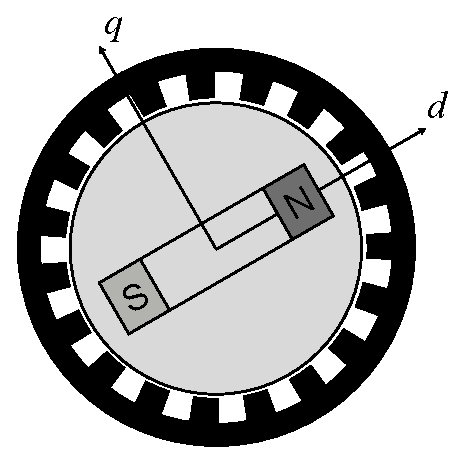
\includegraphics[width=0.5\columnwidth]{Slike/Inkscape/IPMSMsimple.eps}
    \caption{\label{IPMSM} Presek IPMSM stroja.}
\end{figure}


\section{Model IPMSM} \label{motor}

V pogonu se uporablja simetričen trofazni stroj, katerega matematično opišemo v RKS s sledečima enačbama:

\begin{equation} \label{motorModelD}
    u_d = R_si_d+L_d\frac{di_d}{dt}-\underbrace{\omega L_qi_q}_{e_d}
\end{equation}

\begin{equation} \label{motorModelQ}
    u_q = R_si_q+L_q\frac{di_q}{dt}+\underbrace{\omega L_di_d + \omega\Psi_{TM}}_{e_q}
\end{equation}

, kjer sta $e_d$ in $e_q$ inducirani napetosti vzdolžne in prečne komponente.
\\
Navor, ki ga tvori IPMSM pa je naslednji:

\begin{equation}
    M_{el} = \frac{3}{2}p\Bigl(\underbrace{\Psi_{TM}i_q}_{M_{sinhr}}+\underbrace{(L_d-L_q)i_qi_d}_{M_{rel}}\Bigr)
\end{equation}


%*******************************************************************************
%**                      Brezsenzorsko vodenje FOC                            
%*******************************************************************************
\section{Brezsenzorsko vodenje FOC}

Za poenostavitev vodenja stroja se uporablja Clarkina transformacija s katero trofazne veličine predstavimo v dveh ortogonalnih oseh - $\alpha$ in $\beta$ statorskega koordinatnega sistema (SKS).
Veličine v SKS pa transformiramo v RKS z uporabo Parkove transformacije. Ključna lastnost Parkove transformacije je, da so izmenične statorskega k.s. transformirane v RKS enosmerne. To močno
poenostavi regulacijo faznih tokov. Pri Parkovi transformaciji potrebujemo tudi odklon RKS od SKS, ki se v senzorskih pogonih meri z dajalnikom pozicije, pri brezsenzorskih pa oceni iz merjenih
veličin (tok in napetost). Na sliki \ref{koordinatniSistemSimple} so prikazani koordinatni sistemi, ki se uporabljajo pri FOC vodenju. SKS je poravnan s statorjem, RKS z rotorjem in je od SKS
odklonjen za kot $\theta_r$. Ker pa imamo opravka z brezsenzorskim vodenjem, dejanskega odklona rotorja $\theta_r$ ne poznamo. $\theta_r$ le ocenjujemo in lahko opravimo neko napako ocene. To pomeni,
da regulirane veličine ne bodo v RKS, ampak v drugem koordinatnem sistemu, ki bo od tega zamaknjen. Zamaknjen bo za napako ocene $\Delta\theta$, imenovali pa ga bomo FOC koordinatni sistem (FKS). FKS
je od SKS odklonjen za $\theta_f$. \\
Pomerjeni tokovi stroja se v prvem koraku transformirajo v SKS z uporabo Clarkine transformacije, nato pa s Parkovo v FKS s kotom $\theta_f$. V FKS reguliramo vzdolžni in prečni tok, izhodno napetost
regulatorjev pa transformiramo v trifazne napetosti z inverzno Clarkino in Parkovo transformacijo. Hitrost se regulira z nastavljanjem željega vzdolžnega in prečnega toka.

\begin{figure}[!htbp]
    \centering
    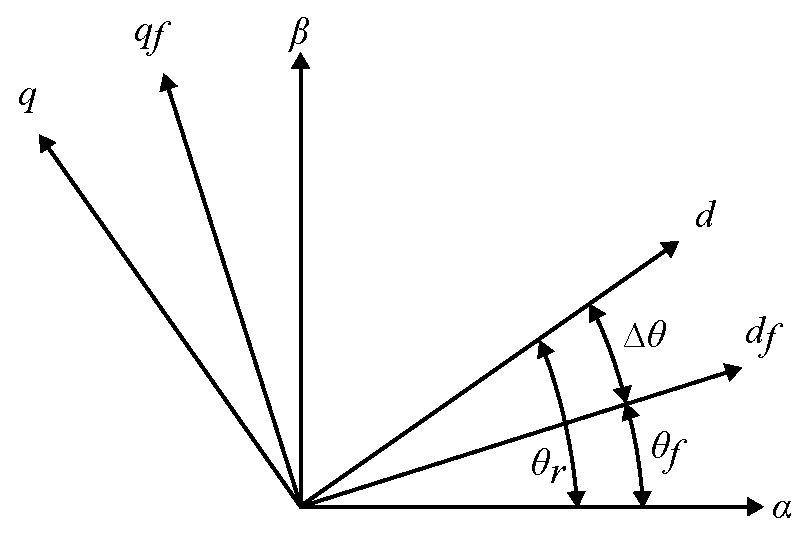
\includegraphics[width=0.7\columnwidth]{Slike/Inkscape/koordinatniSistemSimple.eps}
    \caption{\label{koordinatniSistemSimple} Uporabljeni koordinatni sistemi pri FOC vodenju.}
\end{figure}

Shema na sliki \ref{FOCshema} prikazuje brezsenzorsko vodenje, kjer se odklon in hitrost ocenjujeta, v primeru senzorskega pogona pa bi se merila.

\begin{figure}[!htbp]
    \centering
    \includegraphics[width=1\columnwidth]{Slike/Inkscape/FOCsimple.eps}
    \caption{\label{FOCshema} Shema brezsenzorskega FOC vodenja.}
\end{figure}


%================================================================================
%================================================================================
%**                             Delovanje HFSI                           
%================================================================================
%================================================================================

\chapter{Delovanje HFSI} \label{teorija}

HFSI algoritem temelji na dejstvu, da se induktivnost IPMSM stroja spreminja s pozicijo rotorja. To je ključno za brezsenzorski opazovalnik, saj z merjenjem induktivnosti lahko ocenimo pozicijo
rotorja. Na sliki \ref{induktivnostStroja} je prikazana induktivnost ene faze stroja, pomerjena z RLC metrom.

\begin{figure}[!htbp]
    \centering
    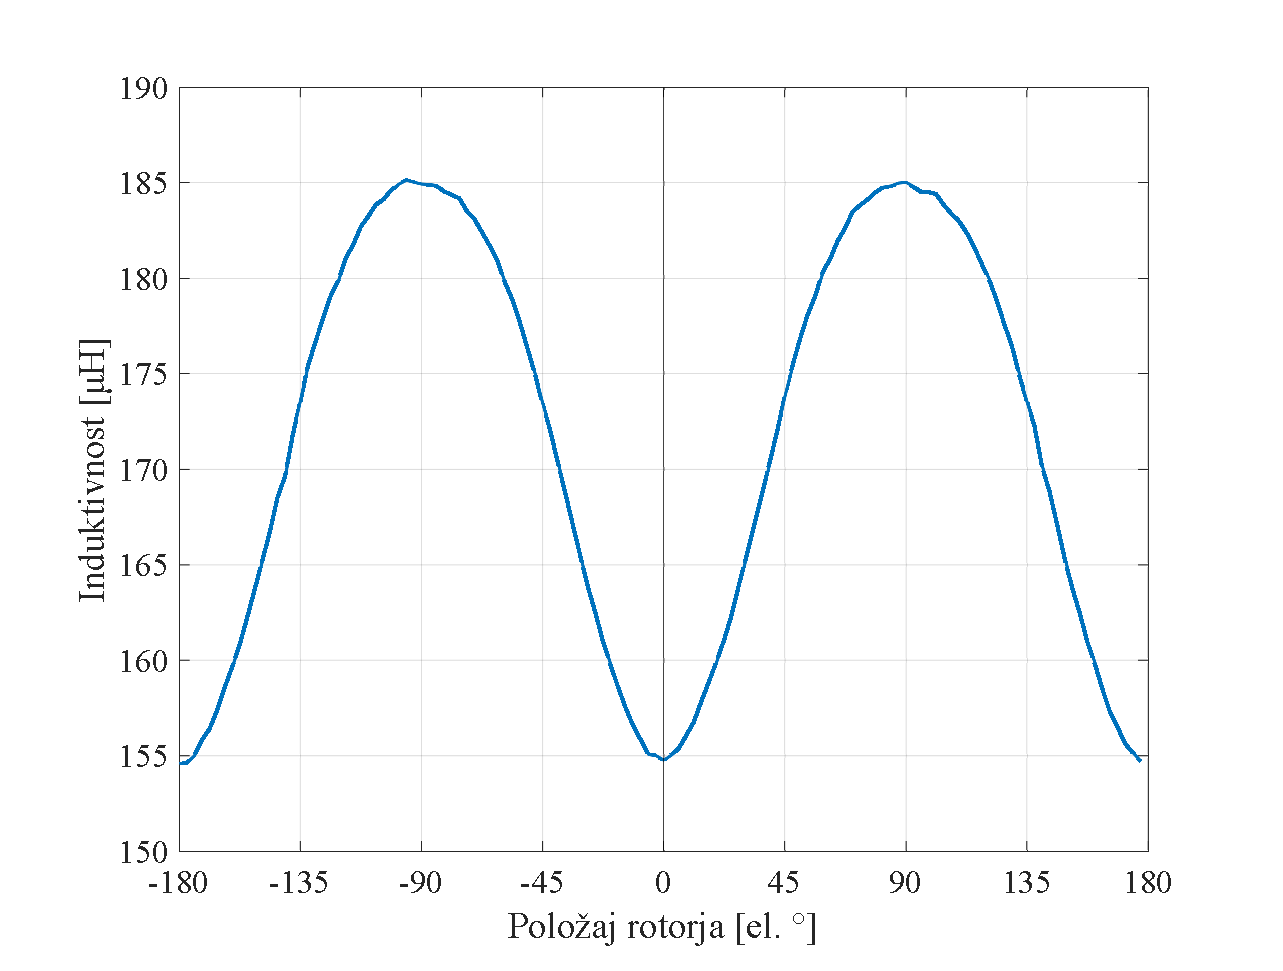
\includegraphics[width=0.72\columnwidth]{Slike/induktivnostStroja.eps}
    \caption{\label{induktivnostStroja} Induktivnost stroja. }
\end{figure}

Induktivnost na sliki je prikazana v odvisnosti od relativne rotorske pozicije. Lahko pa pričakujemo minimalno induktivnost v vzdolžni osi rotorja, saj so v tej osi potopljeni permanentni magneti, ki
imajo mnogokrat manjšo permeabilnost od feromagnetnega materiala rotorja. V prečni osi pa je induktivnost maksimalna. Na vmesnih pozicijah pa je induktivnost nekje med maksimalno in minimalno, oblika
induktivnosti pa je odvisna od geometrije rotorja. Opazimo, da ni striktno sinusoidne oblike.

% Enačba La = Lp + Lr cos(2theta)



%*******************************************************************************
%**                     Visokofrekvenčno vzbujanje statorja                             
%*******************************************************************************
\section{Visokofrekvenčno vzbujanje statorja}

Ker želimo pozicijo ocenjevati preko induktivnosti, je to potrebno na nekakšen način meriti. Pri večini metod se stator vzbuja z napetostnim signalom in se pozicijo ocenjuje direktno iz tokovnega
odziva, brez vmesnega izračuna induktivnosti. Te ni potrebno izračunati, saj je tokovni odziv odvisen od induktivnosti, ta pa od pozicije. Induktivnost vpliva na amplitudo VF tokovnega odziva, zato je
potrebno iz merjenega odziva izločiti amplitudo. To se izvede z uporabo Fourierove vrste \cite{enwiki:fourierSeries}.

Na začetku poglavja je bila prikazana induktivnost stroja, na sliki \ref{tokovniOdzivAlpha} pa je prikazana amplituda tokovnega odziva v $\alpha$ osi. 

\begin{figure}[!htbp]
    \centering
    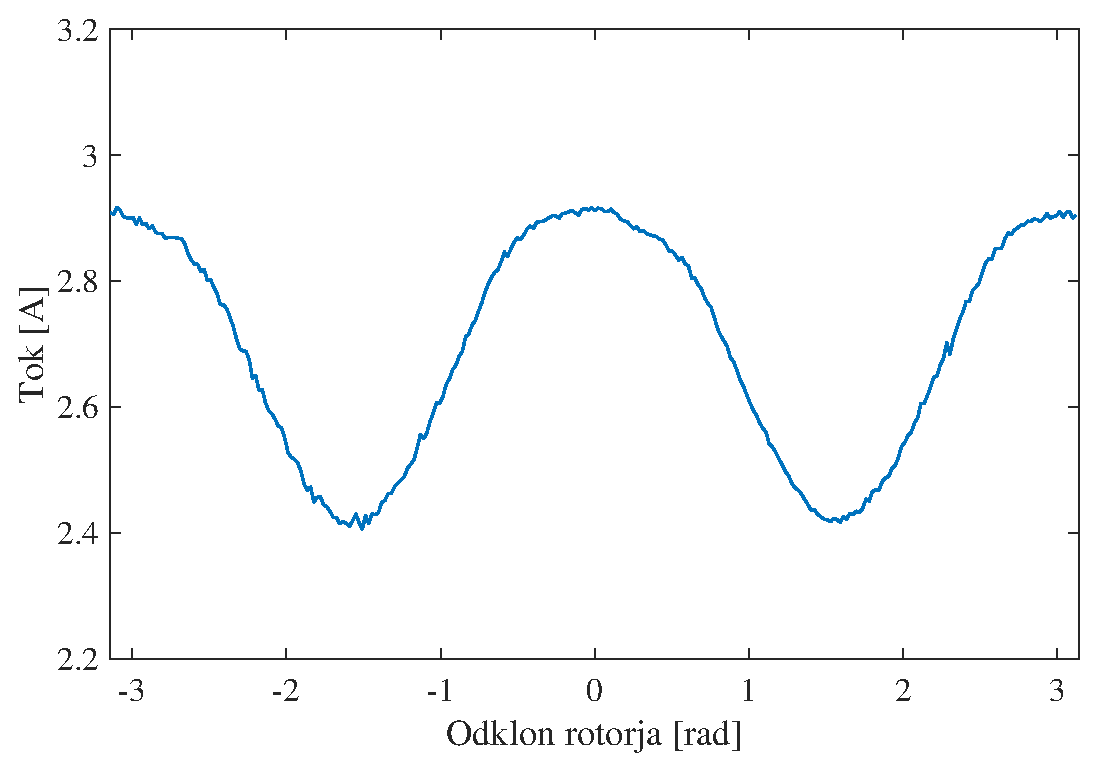
\includegraphics[width=0.9\columnwidth]{Slike/tokovniOdzivAlpha.eps}
    \caption{\label{tokovniOdzivAlpha} Amplituda VF tokovnega odziva v $\alpha$ osi v odvisnosti od pozicije rotorja.}
\end{figure}

Vzbujali smo v SKS, z vrtenjem rotorja prikažemo odvisnost amplitude tokovnega odziva od pozicije rotorja. Opazimo, da je kot induktivnost tudi amplituda približno sinusoidne oblike z dvakratno
frekvenco rotorske pozicije. Amplituda ima maksimalno vrednost, ko je vzdolžna os rotorja poravnana z $\alpha$ osjo oziroma, ko ima rotor odklon 0 stopinj (in 180°). Ko pa je z $\alpha$ osjo 
poravnana prečna os rotorja, je amplituda minimalna.  

Iz amplitude tokovnega odziva prikazanega na sliki \ref{tokovniOdzivAlpha} bi težko ocenili pozicijo rotorja, saj funkcija amplitude odziva ni enolična preslikava pozicije. Če bi bila amplituda
tokovnega odziva pri vsaki poziciji unikatna, bi potrebovali le obratno funkcijo, s katero bi prišli do pozicije. Na sliki \ref{tokovniOdzivAlphaBeta} je prikazan še odziv v $\beta$ osi. Opazimo, da
je podoben odzivu v $\alpha$ osi, le fazno zamaknjen za $\frac{\pi}{2}$. 

\begin{figure}[!htbp]
    \centering
    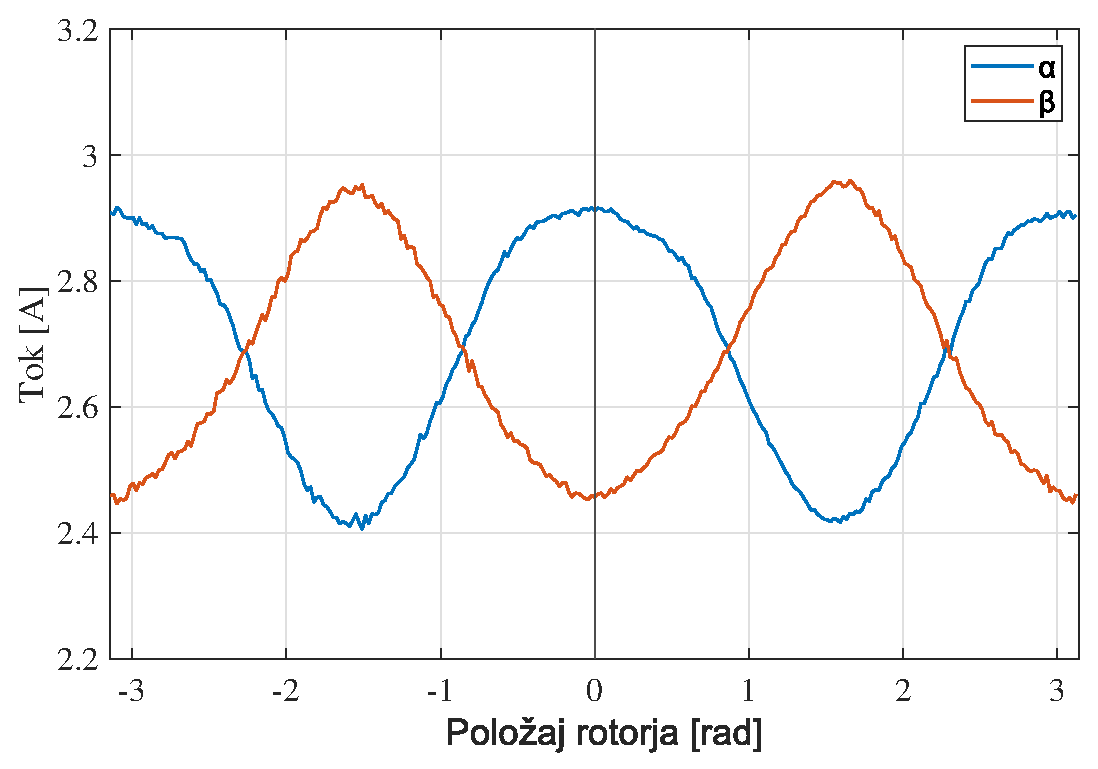
\includegraphics[width=0.9\columnwidth]{Slike/tokovniOdzivAlphaBeta.eps}
    \caption{\label{tokovniOdzivAlphaBeta} Amplituda VF tokovnega odziva v oseh $\alpha$ in $\beta$ v odvisnosti od pozicije rotorja.}
\end{figure}

Tudi z dodatnim odzivom v $\beta$ osi bi bilo ocenjevanje pozicije rotorja iz teh dveh odzivov še vedno težavno. Če bi odziva odšteli, da se znebimo enosmerne komponente odziva, bi dobili kosinusoidno
funkcijo. Iz te pa prav tako ne bi mogli izračunati pozicije. 

Lahko pa iz slike \ref{tokovniOdzivAlphaBeta} opazimo, da sta amplitudi odzivov na štirih pozicijah enaki. Če bi lahko sledili eni od teh točk, bi lahko s tem ocenjevali pozicijo rotorja. To drži, saj
je pozicija, kjer imata amplitudi enako vrednost relativno na rotor vedno enaka. Vendar pa z vzbujanjem v SKS ($\alpha$ in $\beta$) tega ne moremo doseči, saj ne vzbujamo relativno na rotor ampak na
stator. Za vzbujanje relativno na rotor potrebujemo vzbujanje izvajati v rotorskem koordinatnem sistemu in ne statorskem. Pri FOC vodenju to že izvajamo - v FKS vodimo enosmerne komponente prečnega in
vzdolžnega toka. 

Za lažje razumevanje predpostavimo, da stator vzbujamo v FKS samo z VF signalom. Če FKS poravnamo s SKS in vrtimo rotor, dobimo enak odziv kot na sliki \ref{tokovniOdzivAlphaBeta}, saj sta vzdolžna in
prečna os v tem primeru poravnani z $\alpha$ in $\beta$. Ker z vrtenjem rotorja RKS odklanjamo od FKS, s tem ustvarjamo napako ocene pozicije. To pomeni, da si graf na sliki
\ref{tokovniOdzivAlphaBeta} lahko predstavljamo tudi kot amplitudo VF tokovnega odziva v FKS, v odvisnosti od napake ocenjene pozicije rotorja, $\Delta\theta$. Če pa bo med vrtenjem rotorja FKS
poravnan z RKS, pa bosta amplitudi konstantni. Iz slike \ref{tokovniOdzivAlphaBeta} lahko opazimo, da bo njuna vrednost v vzdolžni osi maksimalna, v prečni pa minimalna. 

Za ocenjevanje pozicije bi lahko poskrbeli, da sta amplitudi maksimalno odmaknjeni. Ker bo v tem primeru FKS poravnan z RKS, bo napaka ocene pozicije enaka 0. Vendar bi bilo ohranjanje maksimalne
razlike amplitud VF tokovnih odzivov kompleksen problem, saj ob neki napaki ocene pozicije in tako s prehodom izven maksimalne razlike amplitud v manjšo razliko težko vemo, ali je napaka ocene
pozitivna ali negativna. To pa pomeni, da ne vemo v katero smer moramo popraviti pozicijo, da pridemo nazaj na maksimalno razliko amplitud.

Zato želimo doseči, da sta amplitudi VF tokovnega odziva v prečni in vzdolžni smeri enaki oziroma njuna razlika enaka nič. Ob neki napaki, njuna razlika ne bo več ničta, ampak bo ob pozicitivni napaki pozitivna, ob negativni pa
negativna. S tem bomo razlikovali smer napake in bili zmožni popraviti napako v nasprotno smer. 

Amplitudi VF tokovnega odziva bosta imeli enako vrednost, ko bo FKS od RKS odmaknjen za $\frac{\pi}{4}$. Iz tega pa sledi, da bomo imeli $\frac{\pi}{4}$ napake v oceni pozicije rotorja. Ta problem
rešimo tako, da uvedemo nov koordinatni sistem - HFSI k.s. (HKS). V tem koordinatnem sistemu bomo vzbujali stator z VF napetostnim signalom in merili VF tokovni odziv. Preko amplitude tokovnega odziva
bomo popravljali odklon HKS, da bosta amplitudi VF tokovnega odziva enaki. Ker bosta amplitudi enaki takrat, ko bomo s HKS od RKS odmaknjeni za $\frac{\pi}{4}$, FKS od HKS odmaknjemo za
$\frac{\pi}{4}$. 

Na sliki \ref{koordinatniSistem} je prikazan nov koordinatni sistem HKS poleg RKS in FKS. Prikazana je tudi ovojnica amplitude VF tokovnega odziva v polarnih koordinatah, z vektorji pa je označena
meritev amplitude v prečni in vzdolžni osi HKS. 

\begin{figure}[!htbp]
    \centering
    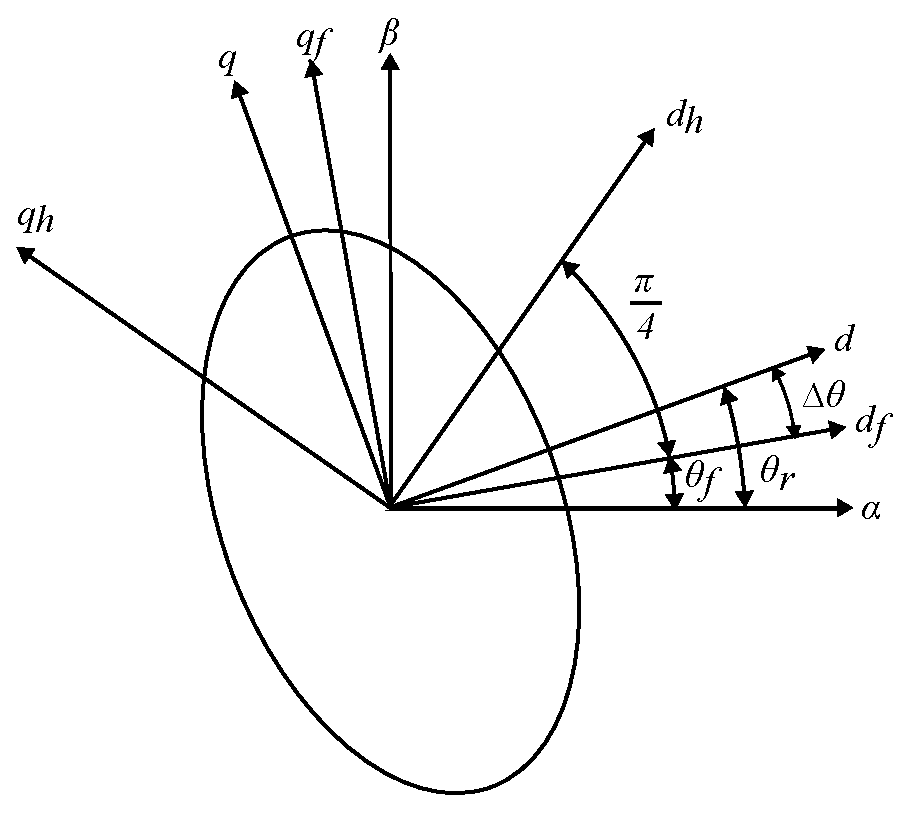
\includegraphics[width=0.7\columnwidth]{Slike/Inkscape/koordinatniSistem.eps}
    \caption{\label{koordinatniSistem} Koordinatni sistemi RKS z amplitudo VF tokovnega odziva v črni, FKS v modri in HKS v rdeči v barvi. Prikazani sta tudi amplitudi VF tokovnega odziva $I_{dh}$ in $I_{qh}$.}
\end{figure}

%*******************************************************************************
%**                      Izračun pozicije rotorja                               
%*******************************************************************************
\newpage
\section{Izračun pozicije rotorja}

Za minimizacijo napake ocene pozicije potrebujemo torej poskrbeti, da imata amplitudi VF tokovnega odziva v prečni in vzdolžni osi enako vrednost, torej mora biti njuna razlika nič. 
Zato uvedemo novo spremenljivko $I_e$, definirano z enačbo \ref{CalcIe}.

\begin{equation} \label{CalcIe}
    I_e = I_{dh} - I_{qh}
\end{equation}

Na sliki \ref{reguliranaVelicinaIdq0} je prikazan tok $I_e$, v odvisnosti od odklona FKS od RKS, oziroma napake ocene pozicije $\Delta\theta$. 

\begin{figure}[!htbp]
    \centering
    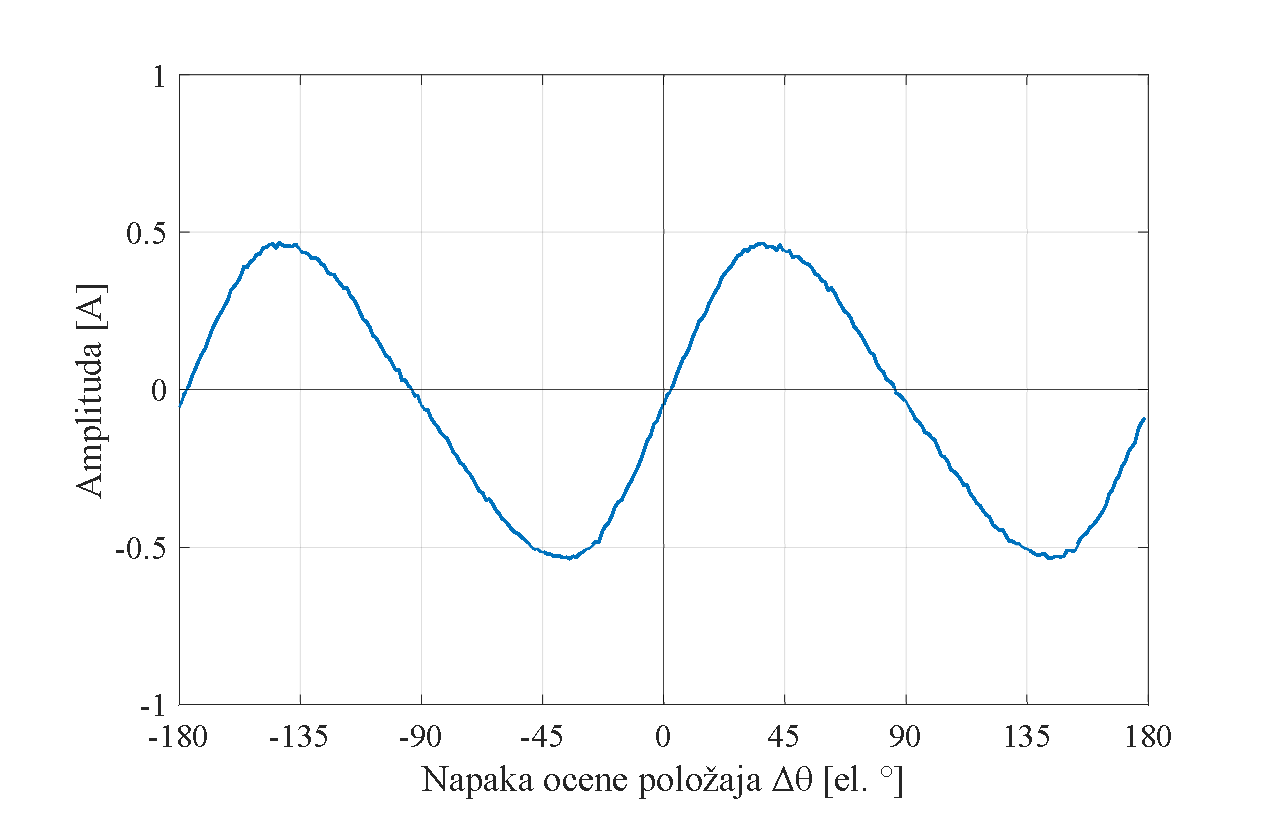
\includegraphics[width=0.9\columnwidth]{Slike/reguliranaVelicinaIdq0.eps}
    \caption{\label{reguliranaVelicinaIdq0} $I_e$ v odvisnosti od odklona FKS od RKS.}
\end{figure}

Pri tej meritvi je bil HKS od FKS odmaknjen za $\frac{\pi}{4}$, FKS pa je bil poravnan z SKS. Z vrtenjem rotorja smo prikazali odvisnost $I_e$ od napake ocene pozicije $\Delta\theta$. 

Ko je ocena brez napake, je razlika amplitud VF tokovnega odziva v prečni in vzdolžni osi enaka nič. Opazimo tudi, da se $I_e$ okoli željene vrednosti z napako spreminja dokaj linearno. S PI
regulatorjem lahko reguliramo $I_e$ in s tem ocenjujemo odklon HKS.

Od željene vrednosti $I_e$ - nič - odštejemo dejansko vrednost in to vstavimo v PI regulator. Z izhodom regulatorja želimo vplivati na odklon HKS, saj bomo tako poskrbeli, da bo tok $I_e$ imel željeno
vrednost. V našem primeru bo izhod regulatorja vrtilna hitrost $\omega_h$. To integriramo, da dobimo pozicijo HKS, katero v povratni zanki uporabimo za nov izračun $I_e$. 

Tako z regulacijo $I_e$ na nič dosežemo, da sta amplitudi tokovnega odziva v vzdolžni in prečni komponenti HKS enaki. S tem pa bo odklon HKS od RKS enak $\frac{\pi}{4}$. Ker ocenjujemo pozicijo RKS,
do te pridemo z izračunom:

\begin{equation}
    \theta_{f} = \theta_{h} - \frac{\pi}{4}
\end{equation}

In velja,

\begin{equation}
    I_e = 0 \Rightarrow \theta_{f} = \theta_{r}
\end{equation}
Točke, kjer ima $I_e$ vrednost 0, lahko imenujemo stabilne točke, saj se z odklonom izven tega območja zaradi regulatorja premaknemo nazaj v stabilnost. Na sliki \ref{reguliranaVelicinaIdq0} opazimo,
da so štiri točke kjer je $I_e$ enak nič, na pozicijah $k\frac{\pi}{2}$, kjer je $k$ poljubno celo število. Pri 0 in $\pi$ je naklon $I_e$ pozitiven in se regulator lahko stabilizira v katerikoli od
teh dveh točk. Če se stabiliziramo v točki $\pi$, bo pozitivna enosmerna komponenta v FKS iz vidika rotorja v RKS postala negativna in se bo motor vrtel v nasprotno smer, zato moramo poskrbeti, da se
ujamemo v pravilno stabilno točko. Točki na pozicijah, kjer je naklon $I_e$ negativen pa sta labilni točki, saj ju bo regulator ob vsaki motnji potisnil nazaj v stabilni točki na pozicijah 0 ali
$\pi$.

\newpage
Na sliki \ref{HFSIsimple} je prikazana shema HFSI algoritma. Poleg ocenjevanja pozicije rotorja je prikazano še VF napetostno vzbujanje, ki se z inverzno Parkovo transformacijo iz HKS transformira v
SKS.

\begin{figure}[!htbp]
    \centering
    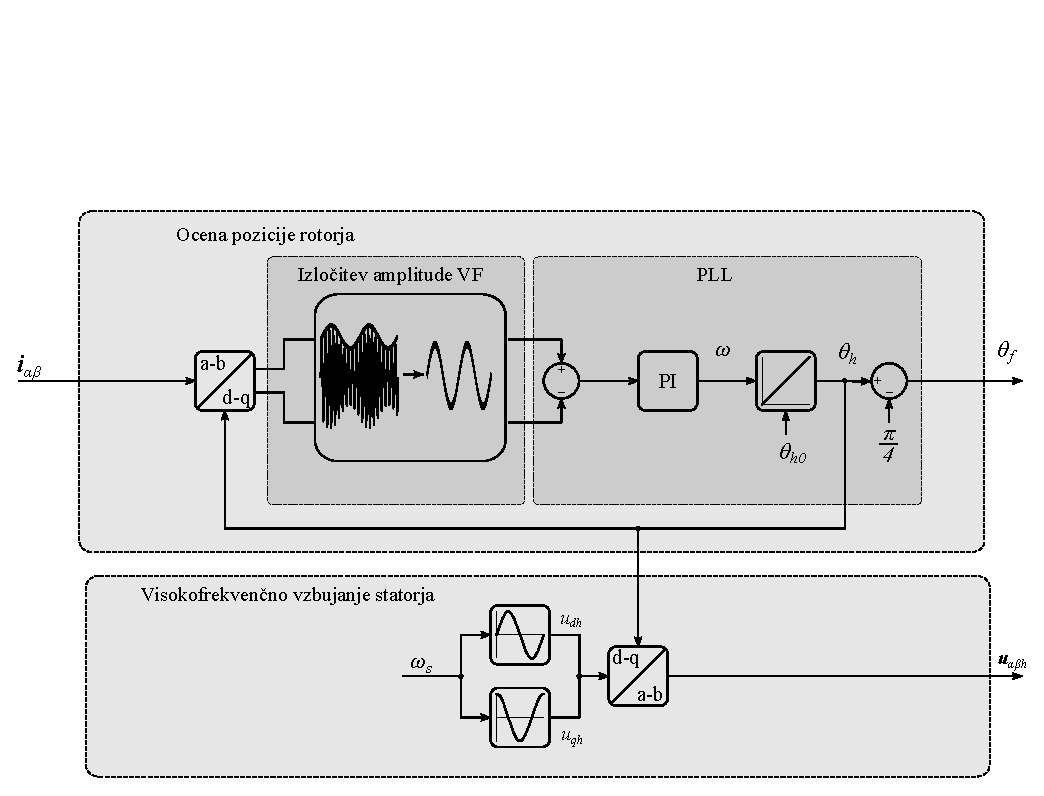
\includegraphics[width=0.9\columnwidth]{Slike/Inkscape/HFSIsimple.eps}
    \caption{\label{HFSIsimple} Shema HFSI algoritma.}
\end{figure}
\newpage
%*******************************************************************************
%**                      Odstopanja realnega sistema                           
%*******************************************************************************
\section{Odstopanja realnega sistema}

Tekom razvoja smo opazili, da amplitudi VF tokovnega odziva v prečni in vzdolžni osi in s tem tok $I_e$ v določenih razmerah začnejo odstopati od pričakovanih. Že na sliki \ref{tokovniOdzivAlphaBeta} 
lahko opazimo, da obliki potekov amplitude v nista enaki. Dodatno lahko opazimo spremembo v oblikah potekov amplitud VF tokovnih odzivov z odklanjanjem HKS relativno na SKS. Na sliki
\ref{tokovniOdzivAlphaBeta} smo vzbujanje izvajali v SKS. To je matematično enako, kot da bi rekli, da smo vzbujanje izvajali v HKS, ki ga poravnamo s SKS. Če pa HKS od SKS odklonimo za
$\frac{\pi}{4}$, bi pričakovali enak odziv kot na sliki \ref{tokovniOdzivAlphaBeta}, le fazno zamaknjen za $\frac{\pi}{4}$. Meritve pa kažejo na to, da se spremeni tudi oblika odziva.

Slika \ref{reguliranaVelicinaIdq0in45} prikazuje primerjavo toka $I_e$ v odvisnosti od rotorske pozicije za dva primera. V prvem primeru je HKS poravnan z SKS, v drugem pa je od njega odmaknjen za
$\frac{\pi}{4}$. Z vrtenjem rotorja prikažemo odvisnost $I_e$ od rotorske pozicije. Odziva sta fazno poravnana za lažjo obravnavo. Opazimo, da se s spremembo oblike premakne stabilna točka. Lahko
pričakujemo, da bomo imeli napako v toku $I_e$ v odvisnosti od odklona HKS od SKS.

\begin{figure}[!htbp]
    \centering
    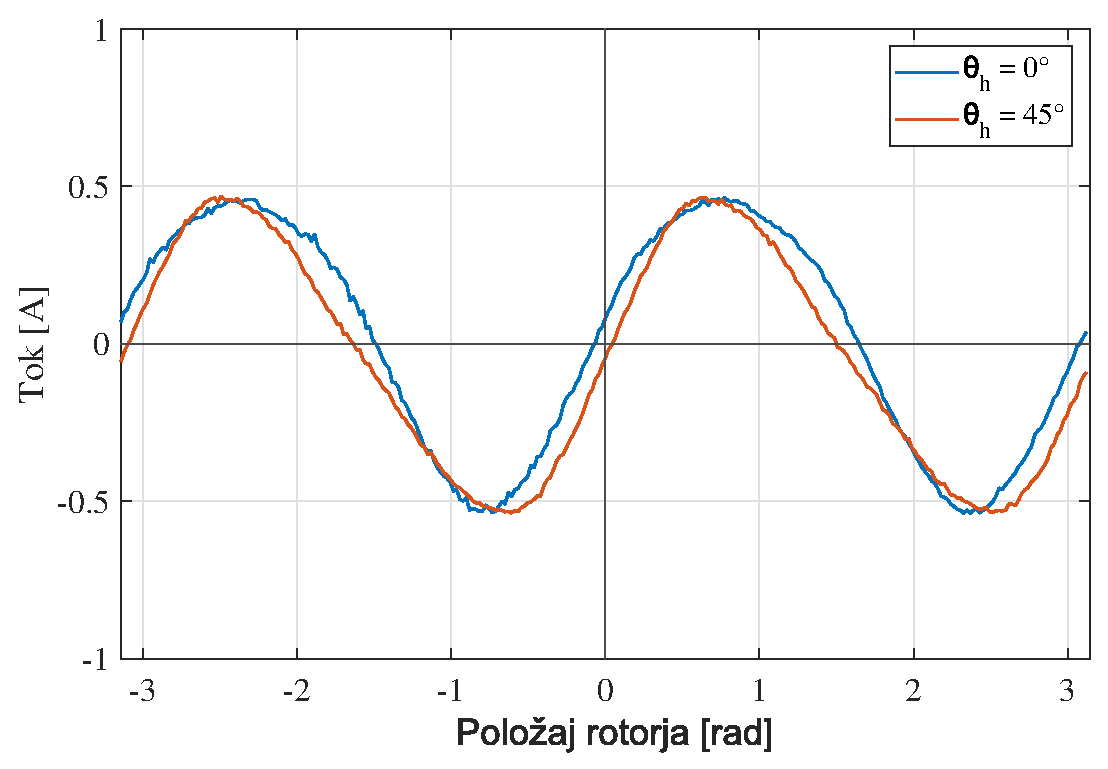
\includegraphics[width=0.88\columnwidth]{Slike/reguliranaVelicinaIdq0in45.eps}
    \caption{\label{reguliranaVelicinaIdq0in45} $I_e$ pri odklonu HKS od FKS 0 in 45°.}
\end{figure}

Na sliki \ref{reguliranaVelicinaIdq0in45} je bila enosmerna komponenta prečnega in vzdolžnega toka nič, stator smo vzbujali le z VF signalom za ocenjevanje pozicije. Za tvorjenje navora pa potrebujemo
neničelno enosmerno prečno komponentno, katere vpliv na tok $I_e$ je prikazan na sliki \ref{reguliranaVelicinaIs}. 
\newline
\begin{figure}[!htbp]
    \centering
    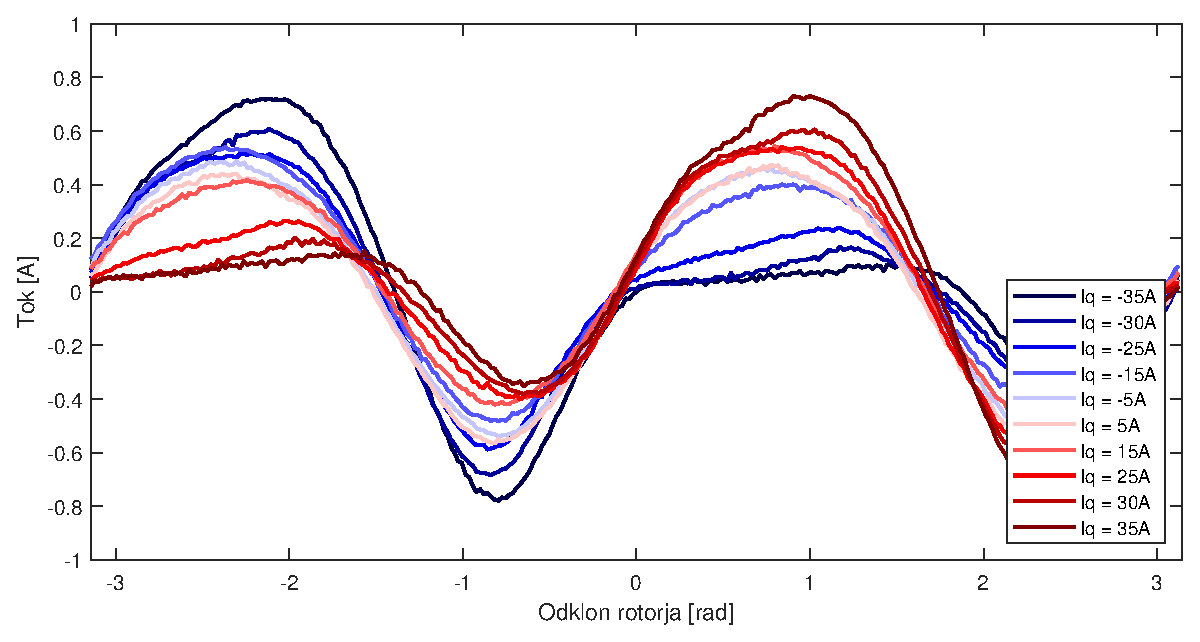
\includegraphics[width=0.85\columnwidth]{Slike/reguliranaVelicinaIs.eps}
    \caption{\label{reguliranaVelicinaIs} Vpliv enosmerne prečne tokovne komponentne na $I_e$ pri različnih odklonih rotorja od FKS.}
\end{figure}

Pri tem eksperimentu je bil FKS poravnan s SKS, rotor pa smo vrteli. Enosmerna prečna komponenta toka je bila vodena s FOC regulatorji toka v koordinatnem sistemu FKS, željena vrednost vzdolžne
komponente pa je bila nič. Enosmerna komponenta vzdolžnega toka je bila v FKS enaka nič, v RKS pa ne, saj smo z odklanjanjem rotorja RKS odmaknili od FKS in se prečna komponenta v FKS preslika v
prečno in vzdolžno komponento RKS. Na sliki se vidi, da z višanjem prečne komponente postane v določenih smereh $I_e$ bolj izrazit v drugih pa bolj položen. Bolj pomembno pa je spreminjanje oblike in
naklona $I_e$ okoli stabilne točke, kjer bo delovna točka našega sistema. Z nekim odstopom okoli ničelne napake se bo $I_e$ premikal po krivulji, prikazani na sliki. Sprememba naklona pomeni spremembo
ojačanja povratne zanke, to pa pomeni spremembo dinamike sistema. Naklon se s pozitivnim prečnim tokom sicer ne spreminja, lahko pa opazimo, da se z negativnim prečnim tokom (ko želimo stroj vrteti v
nasprotno smer) $I_e$ okoli delovne točke ne spreminja linearno. To nam lahko okvari delovanje in terja postavitev delovne točke v drugo stabilno lego.

Dodatna meritev, kjer se odstopanje realnega sistema dobro opazi je, ko FKS poravnamo z RKS, katerega odklon je merjen z dajalnikom pozicije. Pričakovali bi, da bi bila $I_e$ z vrtenjem rotorja (RKS)
na vseh pozicijah enaka nič, saj v tem primeru nimamo napake ocene. Realna meritev pa pokaže na pojav višjeharmonskega popačenja, kot je prikazano na sliki
\ref{tokovniOdzivIs_HKSslediRKS_diff}, kjer je bilo opravljenih več meritev pri različnih prečnih tokovih. Opazimo, da višjeharmonsko popačenje narašča z večanjem prečnega toka.

\begin{figure}[!htbp]
    \centering
    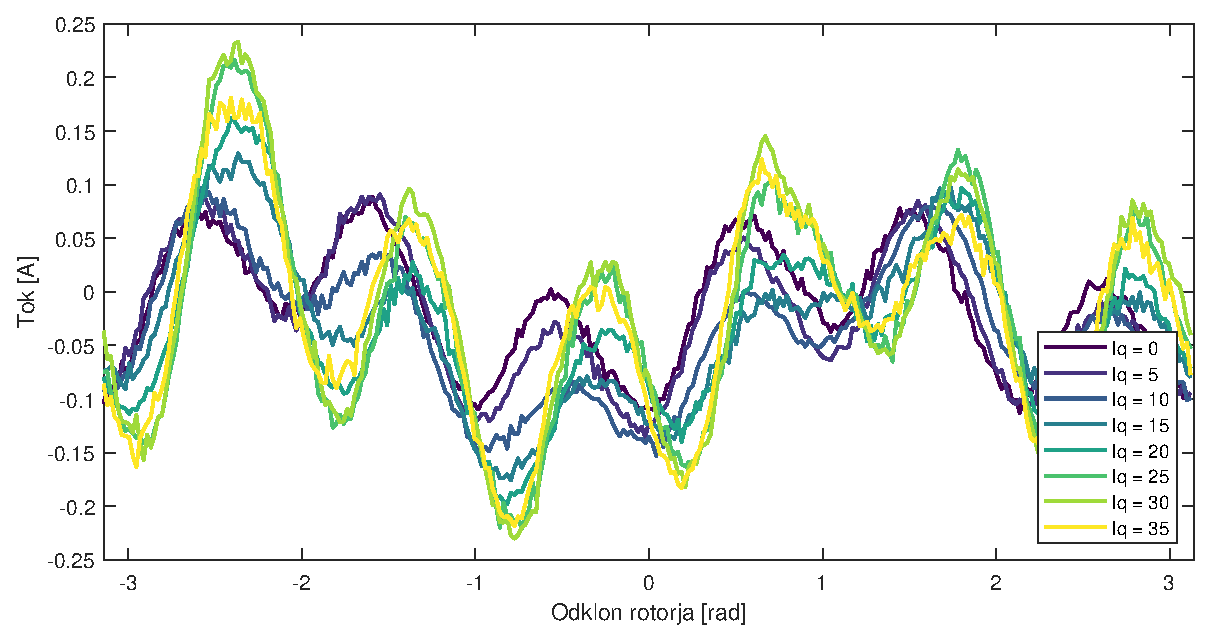
\includegraphics[width=0.95\columnwidth]{Slike/tokovniOdzivIs_HKSslediRKS_diff.eps}
    \caption{\label{tokovniOdzivIs_HKSslediRKS_diff} Neidealnost $I_e$ pri različnih prečnih tokovih, kjer HKS sledi RKS.}
\end{figure}

%*******************************************************************************
%**                      Vpliv mrtvega časa pretvornika                           
%*******************************************************************************
\section{Vpliv mrtvega časa pretvornika}

V praktičnem sistemu se željena izhodna napetost krmilnika pretvori v dejansko z uporabo dvonivojskega pretvornika. Ker ima stroj tri faze, je pretvornik sestavljen iz treh tranzistorskih vej. Primer
ene je prikazan na sliki \ref{mrtviCasRazlaga}. 

\begin{figure}[!htbp]
    \centering
    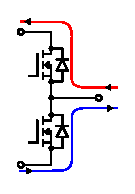
\includegraphics[width=0.4\columnwidth]{Slike/Inkscape/mrtviCasRazlaga.eps}
    \caption{\label{mrtviCasRazlaga} Napetost faze ko sta oba tranzistorja zaprta}
\end{figure}

Da se izognemo hkratnemu prevajanju obeh tranzistorjev, med izklopom zgornjega in vklopom spodnjega vrinemo interval v katerem nobeden od njiju ni
prožen. Temu intervalu pravimo mrtvi čas. Ko teče tok tranzistorske veje v fazo, med mrtvim časom komutira čez diodo spodnjega tranzistorja. V tem času je napetost te faze enaka spodnjem napetostnem
nivoju tranzistorske veje. Ko pa tok komutira čez zgornjo diodo, pa je napetost faze enaka zgornjem napetostnem nivoju. Napetost faze med mrtvim časom je torej odvisna od polaritete toka skozi vejo.
To pomeni, da željena vrednost fazne napetosti ni enaka dejanski \cite{ambrovzivc2016elektrivcni}. 

Za delovanje HFSI algoritma poleg enosmerne komponente toka za tvorjenje navora vzbujamo stator še z visoko frekvenčno komponento. V primeru, kjer stator vzbujamo samo z visoko frekvenco, bi mrtvi čas
vedno vplival na odziv in njegov vpliv bi bil konstanten in enak v prečni in vzdolžni smeri. Ko pa vzbujamo še s konstantnim prečnim tokom, pa mrtvi čas na VF napetostno komponento vpliva samo, ko
tokovni odziv spreminja polariteto. To lahko potrdimo z meritvami na realnem sistemu, kjer poleg VF vzbujanja uporabljamo tudi enosmerno prečno komponentno, rotor pa počasi vrtimo. FKS in RKS
poravnamo, zato bi pričakovali konstantno ničelno vrednost toka $I_e$.

Na sliki \ref{mrtviCas} poleg visokoharmonskega popačenja opazimo, da je na šestih pozicijah odziv popačen in da je magnituda napake dokaj linearno odvisna od mrtvega časa.

\begin{figure}[!htbp]
    \centering
    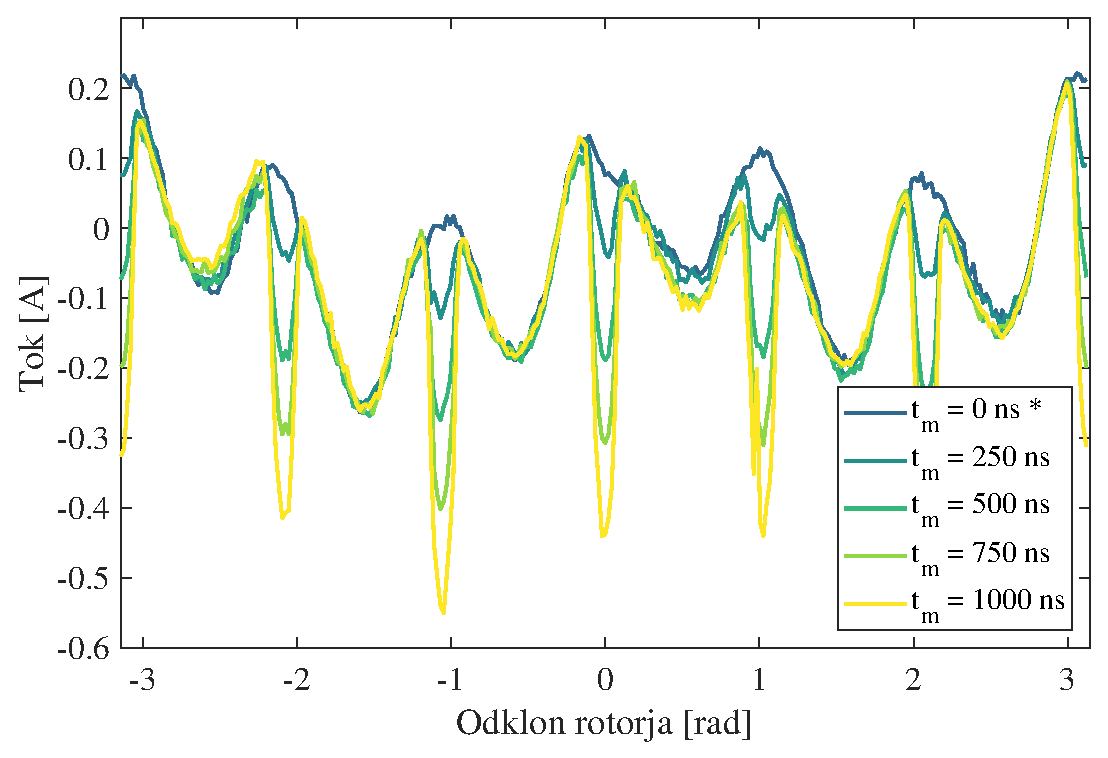
\includegraphics[width=0.8\columnwidth]{Slike/mrtviCas.eps}
    \caption{\label{mrtviCas} Odvisnost popačenja amplitude odziva od dolžine mrtvega časa }
\end{figure}

Prav tako lahko potrdimo, da je mrtvi čas odvisen od napajalne napetosti, prikazano na sliki \ref{mrtviCasNapetost}. Odziv je bil pomerjen pri napajalnih napetostih 16V, 24V in 32V.
\renewcommand*{\thefootnote}{\fnsymbol{footnote}}
\footnotetext[1]{Mrtvi čas v tem primeru ni bil 0 ns, ampak najnižji možen, s katerim efekt mrtvega časa še ni bil viden. Vrednost mrtvega časa je bila v tem primeru približno 100 ns.}
\begin{figure}[!htbp]
    \centering
    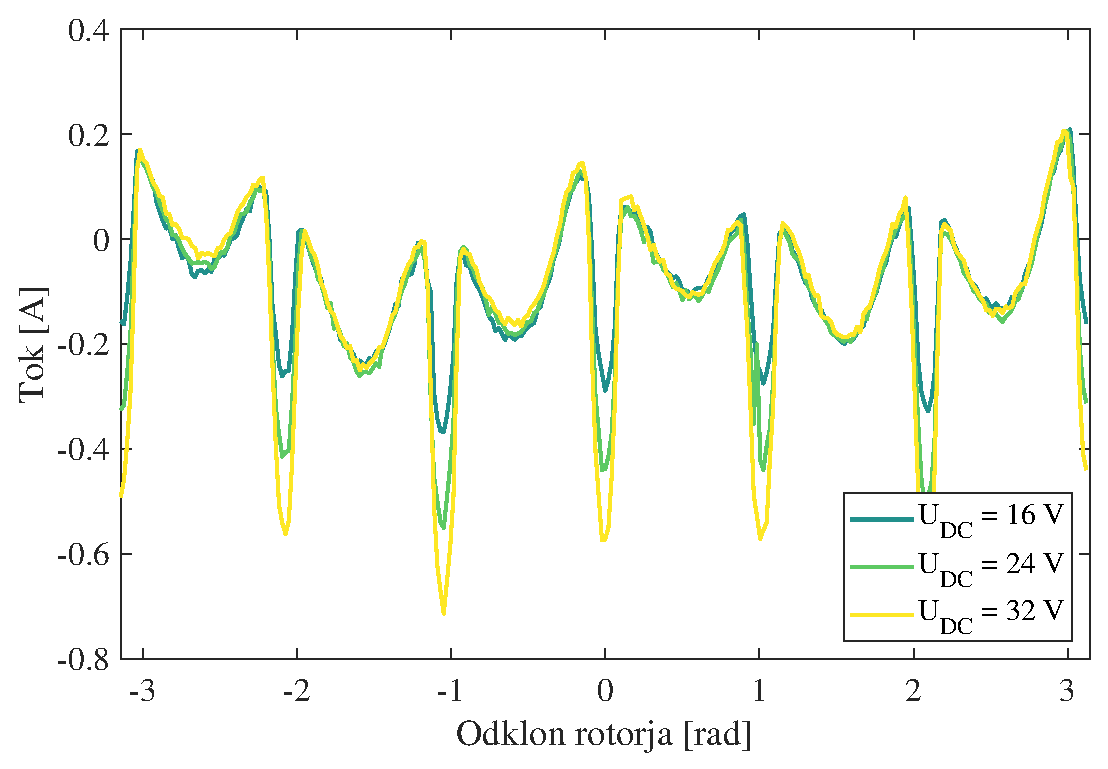
\includegraphics[width=0.8\columnwidth]{Slike/mrtviCasNapetost.eps}
    \caption{\label{mrtviCasNapetost} Odvisnost popačenja amplitude odziva od napajalne napetosti }
\end{figure}


\newpage
Dodatno lahko pokažemo, da se vpliv mrtvega časa začne kazati takrat, ko začne VF tokovni odziv menjati polariteto. Na zgornjem grafu slike \ref{mrtviCasFazniTok} je prikazan fazni tok $i_u$, z
obarvanim delom, kjer menja polariteto. Na drugem grafu sta prikazani amplitudi VF tokovnega odziva v vzdolžni in prečni osi. Opazi se, da mrtvi čas na amplitudi vpliva, ko fazni tok menja polariteto.

\begin{figure}[!htbp]
    \centering
    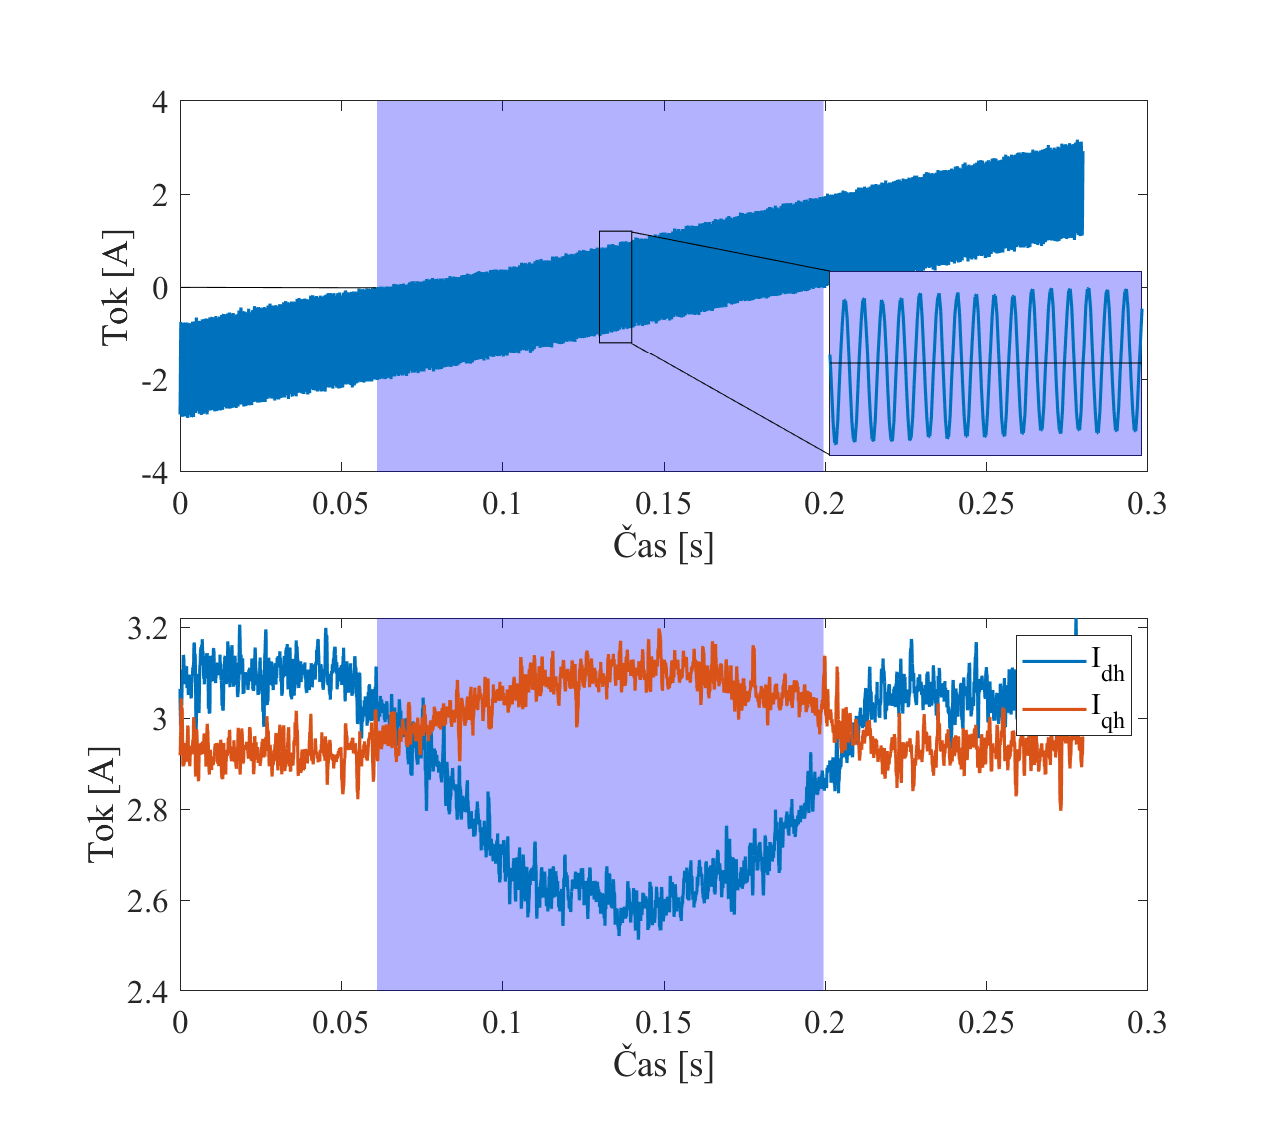
\includegraphics[width=0.9\columnwidth]{Slike/mrtviCasFazniTok.eps}
    \caption{\label{mrtviCasFazniTok} Vpliv mrtvega časa na faznem toku }
\end{figure}

Iz slike \ref{mrtviCasFazniTok} lahko sklepamo, da bo popačenje zaradi mrtvega časa večje, če bo enosmerna komponenta toka v FKS manjša, saj bo VF tokovna komponenta dalj časa menjala polariteto. To
lahko pokažemo z meritvijo, prikazano na sliki 
\ref{tokovniOdzivIs_HKSslediRKS_IdiffAmp_DT}

\begin{figure}[!htbp]
    \centering
    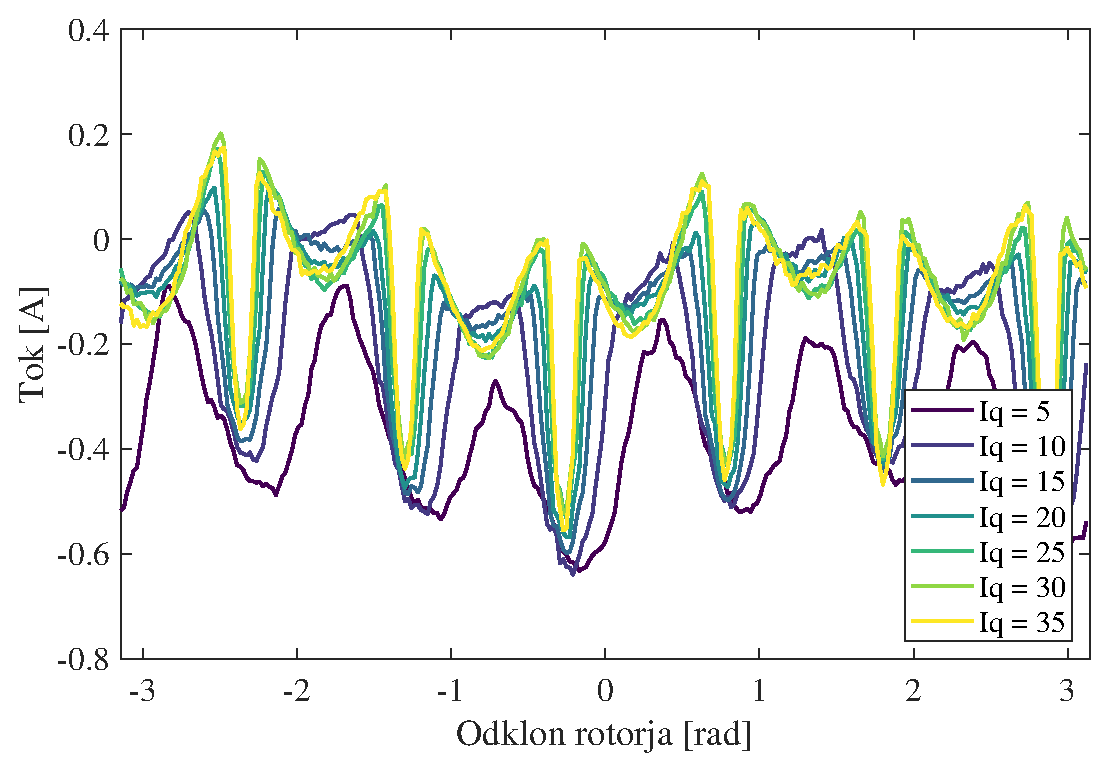
\includegraphics[width=0.75\columnwidth]{Slike/tokovniOdzivIs_HKSslediRKS_IdiffAmp_DT.eps}
    \caption{\label{tokovniOdzivIs_HKSslediRKS_IdiffAmp_DT} Vpliv prečnega toka na popačenje $I_e$ zaradi mrtvega časa. }
\end{figure}

Takšno popačenje amplitude odziva vpliva na oceno pozicije, saj bo PI regulator poiskušal zmanjšati napako in to tako, da bo spremenil odklon HKS na mesto, kjer ima tok $I_e$ vrednost nič.

%================================================================================
%================================================================================
%**                             Integracija v FOC                           
%================================================================================
%================================================================================
\chapter{Integracija v FOC} \label{integracija}

Za uspešno implementacijo HFSI algoritma, ga je potrebno tudi pravilno integrirati v celotno FOC vodenje. Potrebno je poskrbeti za pravilno inicializacijo algoritma, filtriranje tokovne povratne
zanke, zadnji element pa je preklop v delovanje SMO opazovalnika, ko vrtilna hitrost doseže dovolj visoko vrednost. Na koncu je predstavljen postopek uglaševanja PI regulatorja.

%*******************************************************************************
%**                      Inicializacija HFSI                           
%*******************************************************************************
\section{Inicializacija HFSI}

Ker s HFSI algoritmom nismo zmožni ocenjevati polaritete rotorja (ne razlikujemo med odklonom 0° in 180°), potrebujemo za pravilno smer vrtenja poskrbeti, da je začetna pozicija znana. Pred zagonom
HFSI algoritma ocenimo začetno pozicijo rotorja \cite{IPDBoussak}, ki se začne uporabljati že od samega začetka delovanja HFSI. Ker je HKS od RKS odklonjen za $\frac{\pi}{4}$, je začetna vrednost kota
HKS enaka ocenjeni začetni poziciji RKS z odklonom $\frac{\pi}{4}$.

Pri delovanju HFSI tokovna povratna zanka vključuje tudi VF komponento, ki jo je potrebno izločiti, saj lahko regulatorja toka s povratno zanko vplivata na VF odziv. Uporabimo zaporni pasovni
filter (BSF). Filtriranja ne smemo izvesti v SKS, saj je tam VF komponenta različne frekvence, ki je odvisna tudi od vrtilne hitrosti HKS. Zato filtriramo v FKS, kjer ima konstantno frekvenco in sicer
enako vzbujalnem signalu. Ker filtriramo v FKS, pa lahko filtrirane tokove $i_d$ in $i_q$ direktno uporabimo za regulacijo toka. Ob zagonu prvih nekaj period vzbujalnega signala FOC regulatorje
izklopimo, da se prehodni pojav pasovnih filtrov ustali. 

\newpage

Na sliki \ref{HFSI} je prikazana razširjena shema HFSI algoritma. Prikazano je ocenjevanje pozicije rotorja, kjer se odklon HKS $\theta_h$ uporablja za nov izračun $I_e$ in VF vzbujanje v HKS. S
$\theta_h$ izračunamo odklon FKS, v katerem uporabljamo BSF za izločevanje VF komponente v povratni tokovni zanki. Ker uporabljamo dva d-q koordinatna sistema, se uporabljata dve Parkovi
transformaciji.

\begin{figure}[!htbp]
    \centering
    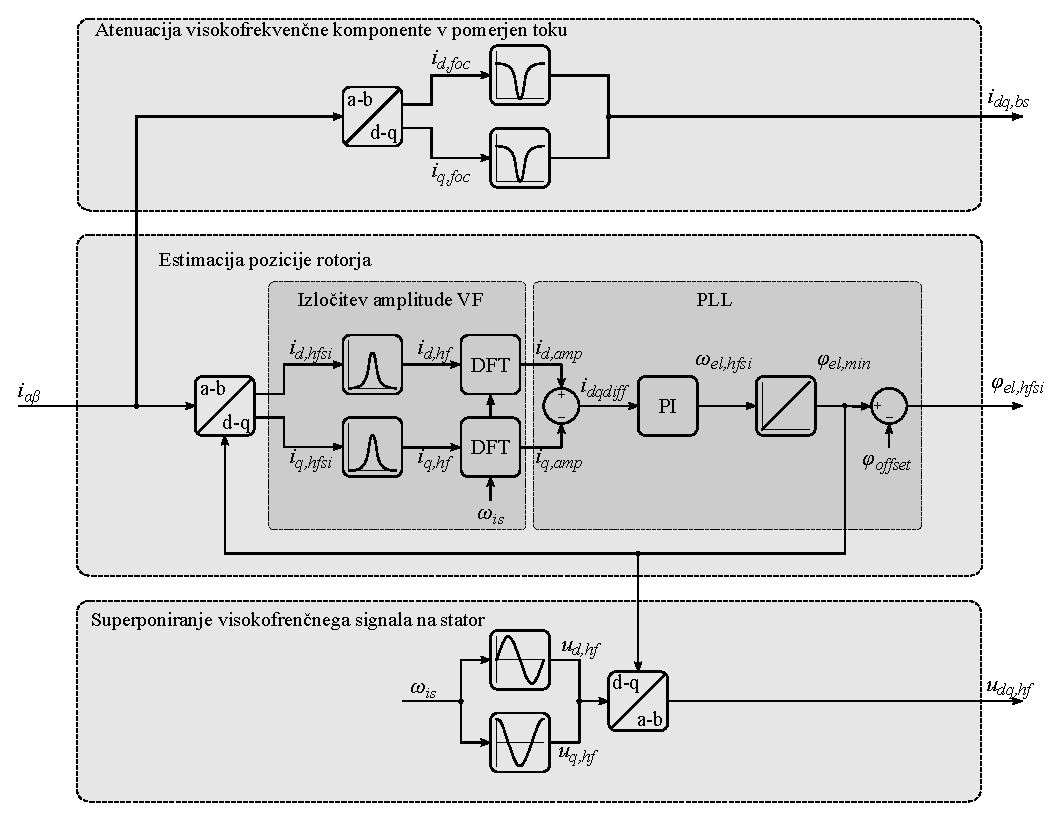
\includegraphics[width=0.95\columnwidth]{Slike/Inkscape/HFSI.eps}
    \caption{\label{HFSI} HFSI shema z dodanim pasovnim filtrom povratne zanke in začetno vrednost integratorja. }
\end{figure}

\newpage

%*******************************************************************************
%**                Brezudarni preklop v delovanje opazovalnika                           
%*******************************************************************************
\section{Brezudarni preklop v delovanje SMO opazovalnika}

Ko je vrtilna hitrost že dovolj visoka, da ocenjujemo pozicijo rotorja z inducirano napetostjo, je potrebno izvesti brezudarni preklop. Takoj po preklopu želimo,
da SMO opazovalnik začne delovati v pravilni delovni točki. To lahko dosežemo tako, da SMO opazovalnik deluje že pred preklopom, vzporedno s HFSI algoritmom. Ob preklopu tako samo izklopimo visokofrekvenčno
vzbujanje statorja. Delovanje SMO opazovalnika vzporedno s HFSI algoritmom pa terja dodatne kalkulacije. Te so lahko v določenih sistemih, kjer je nadvsem pomembna nizka cena in zato uporaba manj
zmogljivih procesorjev previsoke. Zato se uporabi drug način, ki ob preklopu postavi SMO opazovalnik v željeno delovno točko. To pomeni, da je potrebno vsa notranja stanja postaviti na pravilno
začetno vrednost. To vključuje notranja stanja modela, ki se uporabljajo za ocenjevanje inducirane napetosti, ocenjeno hitrost in pozicijo.

Na slikah \ref{brezudarniPreklop_Pos}, \ref{brezudarniPreklop_Speed} in \ref{brezudarniPreklop_Err} so prikazani ocenjena pozicija, hitrost in napaka ocene. Ob preklopu, ki se zgodi okoli 0.5 sekunde,
vrednost hitrosti SMO opazovalnika postavimo na ocenjeno hitrost HFSI algoritma.

\begin{figure}[!htbp]
    \centering
    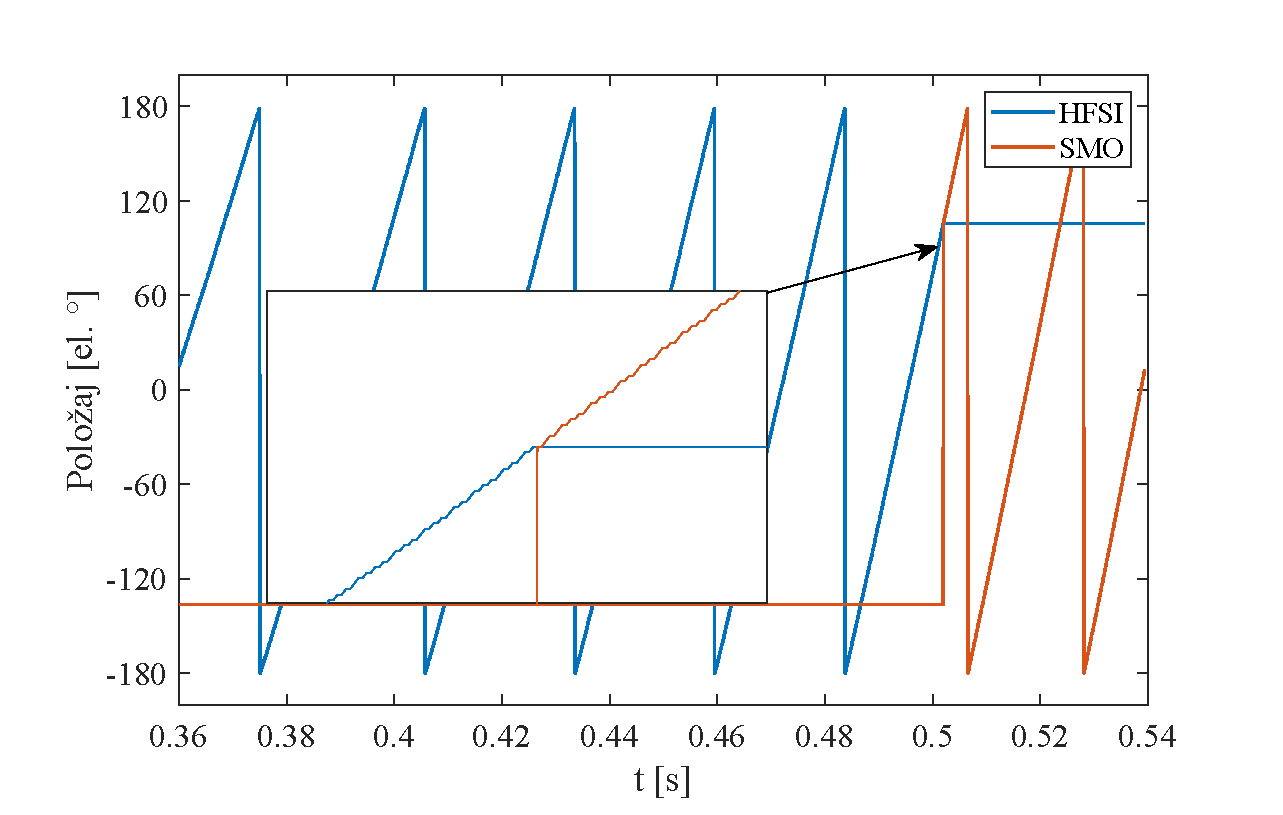
\includegraphics[width=0.8\columnwidth]{Slike/brezudarniPreklop_Pos.eps}
    \caption{\label{brezudarniPreklop_Pos} Preklop v delovanje SMO opazovalnika pozicije. }
\end{figure}

\begin{figure}[!htbp]
    \centering
    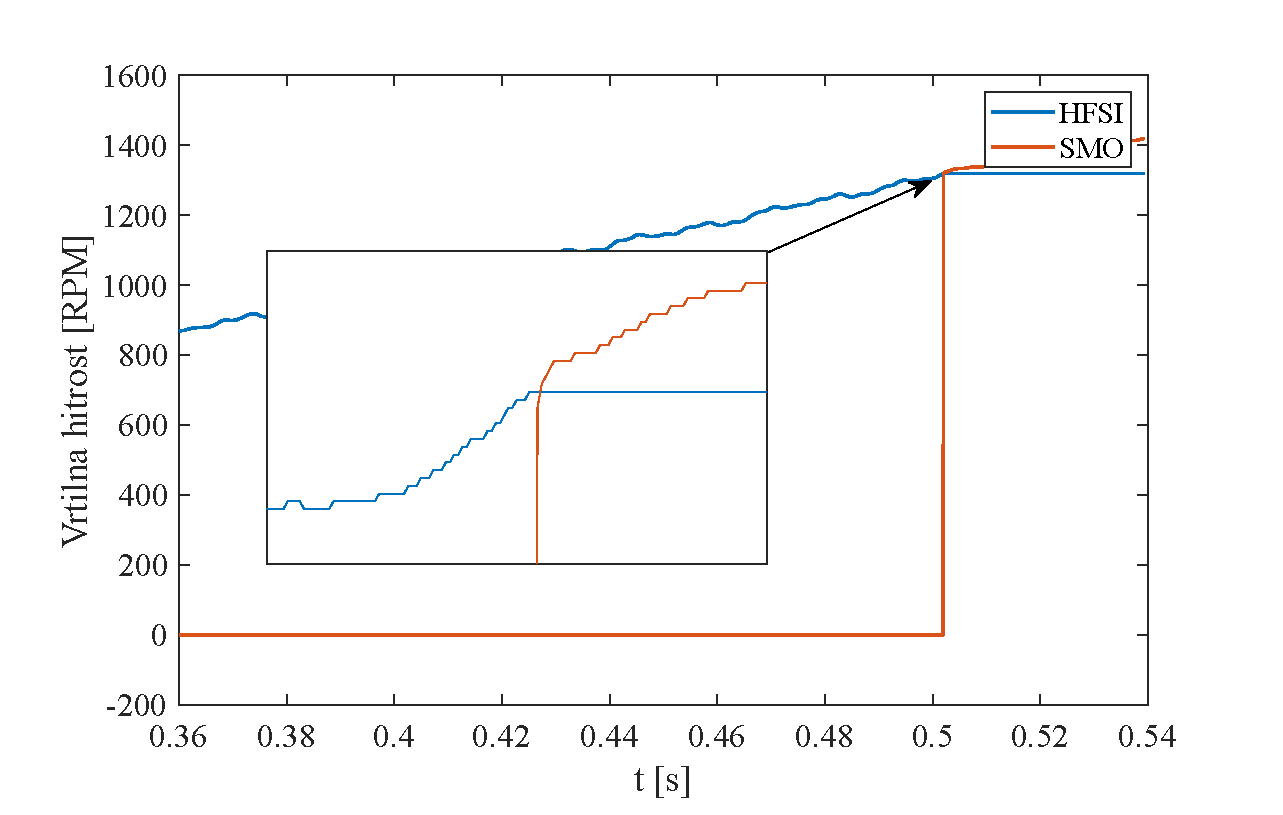
\includegraphics[width=0.8\columnwidth]{Slike/brezudarniPreklop_Speed.eps}
    \caption{\label{brezudarniPreklop_Speed} Preklop v delovanje SMO opazovalnika pozicije. }
\end{figure}

\begin{figure}[!htbp]
    \centering
    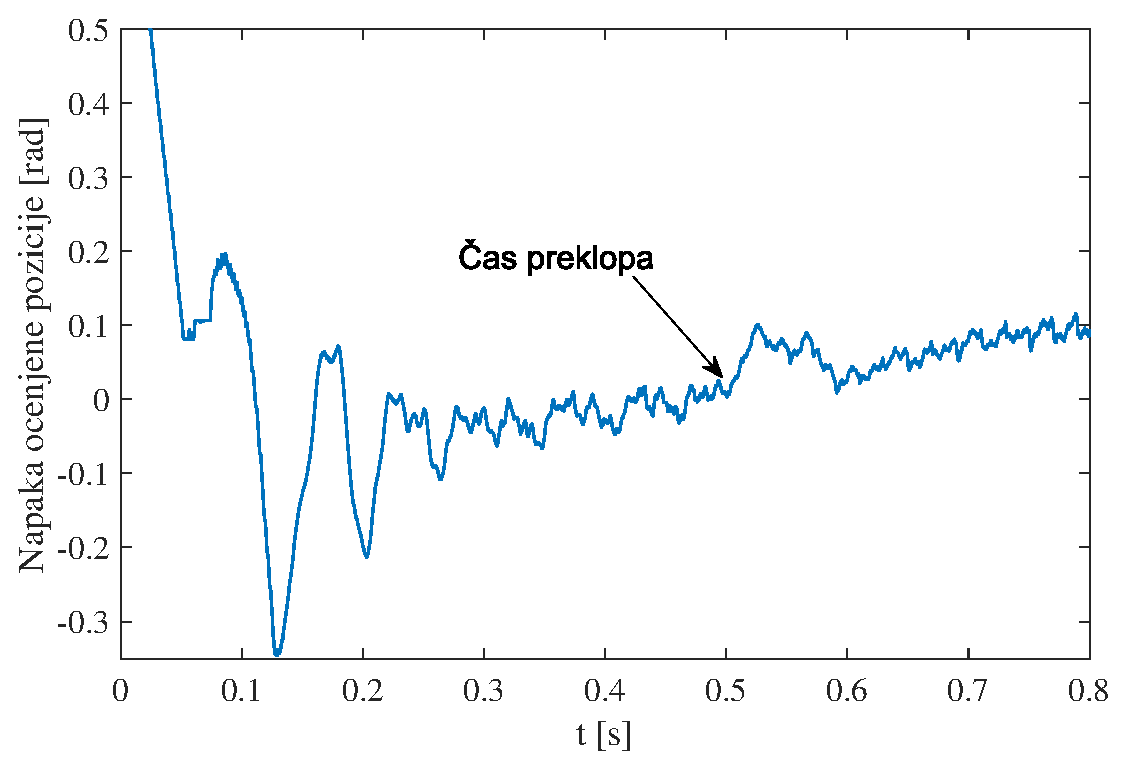
\includegraphics[width=0.8\columnwidth]{Slike/brezudarniPreklop_Err.eps}
    \caption{\label{brezudarniPreklop_Err} Preklop v delovanje SMO opazovalnika pozicije. }
\end{figure}

\newpage
Slika \ref{FOC} prikazuje FOC shemo s HFSI in SMO opazovalnikoma. 

\begin{figure}[!htbp]
    \centering
    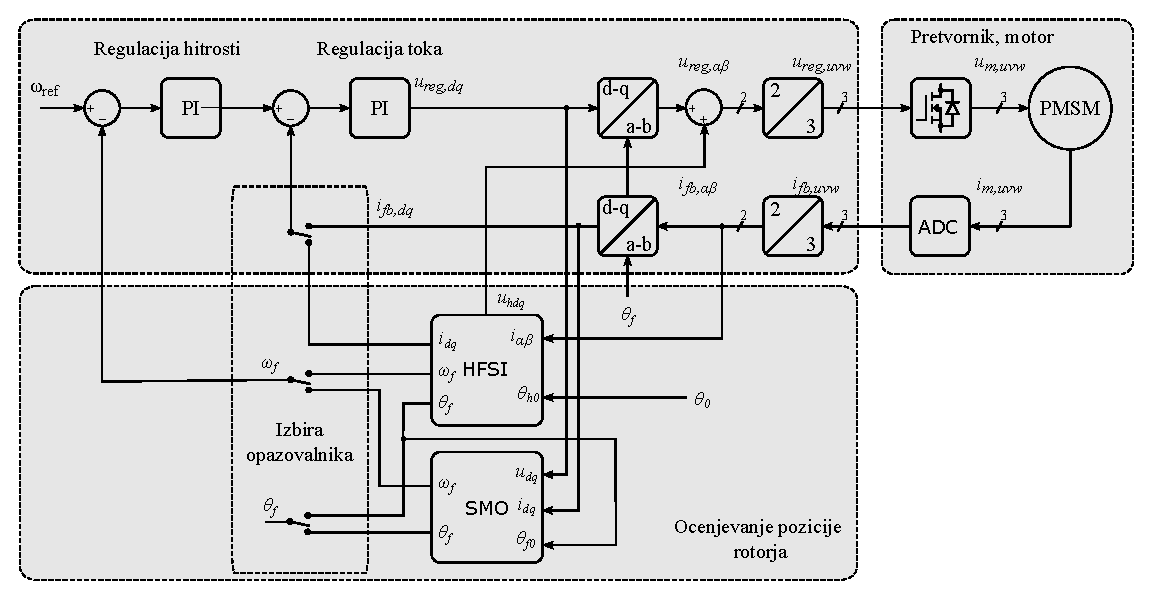
\includegraphics[width=0.95\columnwidth]{Slike/Inkscape/FOC.eps}
    \caption{\label{FOC} FOC shema s HFSI in SMO ocenjevalnikom pozicije. }
\end{figure}

%*******************************************************************************
%**                Nastavitev parametrov PI regulatorja                           
%*******************************************************************************
\newpage
\section{Nastavitev parametrov PI regulatorja}

Parametri regulatorja so bili nastavljeni ročno in sicer z opazovanjem delovanja algoritma pri različnih parametrih. Za kriterijsko funkcijo smo izbrali napako ocenjenega kota in je bila najprej
pomerjena pri desetih različnih $K_p$ parametrih, kjer je imel parameter $K_i$ neko začetno vrednost, pri kateri je bil algoritem stabilen. Nato se je izbral $K_p$ z najmanjšo napako in ponovno pomeril
odziv s tem parametrom in različnimi $K_i$ parametri. Tako smo pridobili $K_p$ in $K_i$ s prvo iteracijo, nato pa se izvedla dodatna iteracija, da smo prišli do optimalnih parametrov. 

V prvi iteraciji je bil obseg vrednosti parametrov, pri katerih se je meril odziv tako, da je algoritem pri robnih vrednostih postal nestabilen. Ko se je izvajala druga iteracija pa se je obseg
parametrov zmanjšal in je bil okoli vrednosti, pridobljene s prvo iteracijo.

Prenizka vrednost $K_p$ parametra povzroči večinoma integralski odziv in dobimo velike dolge prenihaje, prevelika pa popolnoma destabilizira sistem. Prenizek $K_i$ parametrer povzroči desinhronizacijo
stroja. Ko ima $K_i$ dovolj visoko vrednost za sinhrono delovanje stroja, vendar manjšo od optimalne, regulirne veličine nikoli ne zreguliramo na nič, kar povzroči konstantno napako.  Prevelik $K_i$
pa destabilizira sistem.

%================================================================================
%================================================================================
%**                             Eksperimenti                           
%================================================================================
%================================================================================
\chapter{Eksperimenti}  \label{eksperimenti}

V tem poglavju je najprej opisano krmiljenje napetostnega pretvornika in merjenje toka, saj tudi to vpliva na algoritem. Na koncu so prikazane meritve realnega sistema, ki so bile zajete z
osciloskopom, interne spremenljivke, uporabljene v samem algoritmu, pa so bile v realnem času poslane na računalnik preko serijske komunikacije.

\begin{figure}[!htbp]
    \centering
    \includegraphics[width=0.75\columnwidth]{Slike/EksperimentiSlika.jpg}
    \caption{\label{experimentiSlika} Fotografija močnostnega pretvornika in stroja}
\end{figure}

Na fotografiji \ref{experimentiSlika} je prikazan sistem, na katerem je bil razvit HFSI algoritem. 

%*******************************************************************************
%**               Trifazni PWM in meritev toka                         
%*******************************************************************************
\section{Trifazni PWM in meritev toka}

V sistemu se uporablja asimetričen PWM s fazno zamaknjenimi napetostmi. Največja prednost take izvedbe je preprosta implementacija krmiljenja napetosti in merjenja toka, slaba lastnost pa je večje valovanje
faznih tokov s frekvenco PWM-ja. Potek faznih napetosti je prikazan na sliki \ref{PWM}, kjer se vidi fazni zamak faz - fazno sta zamaknjeni druga in tretja faza za merjenje toka. $t_{PWM}$ je perioda PWM, $t_{MEAS}$
pa je časovni zamik poteka faze za tokovno meritev. $t_0$ do $t_5$ pa so časi, kjer faze spremenijo polariteto. Ti časi določajo, kakšna je efektivna napetost na fazah in se izračunajo kot je
prikazano z enačbo \ref{izracunPWM}. $t_0$, $t_1$ in $t_2$ se ne spreminjajo, saj takrat merimo tok, $t_3$, $t_4$ in $t_5$ pa so odvisni od željenih faznih napetosti. Implementacija na mikrokrmilniku
potrebuje še dodatno pretvorbo iz časa v število taktov PWM periferije krmilnika.

\begin{figure}[!htbp]
    \centering
    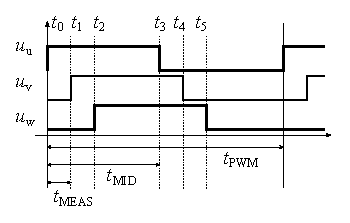
\includegraphics[width=1\columnwidth]{Slike/Inkscape/PWM.eps}
    \caption{\label{PWM} Pulzno širinska modulacija močnostnega pretvornika }
\end{figure}

\begin{equation} \label{izracunPWM}
\begin{gathered}
    t_0 = 0  \\
    t_1 = t_{MEAS}  \\
    t_2 = 2t_{MEAS}  \\
    t_3 = t_{MID} + u_uC  \\
    t_4 = t_{MID} + t_{MEAS} + u_vC \\
    t_5 = t_{MID} + 2t_{MEAS} + u_wC \\
    C = \frac{t_{PWM}}{U_{DC}}
\end{gathered}
\end{equation}

$t_{MID}$ ni polovica $t_{PWM}$, saj smo rezervirali $2t_{MEAS}$ periode za meritev toka. Zato je $t_{MID}$ enak polovici $t_{MID} - 2t_{MEAS}$. $C$ pa je faktor za pretvorbo željenje napetosti v čas
in je preprosto razmerje med dolžino periode in napetostno zalogo. Napetostna zaloga - oziroma napajalna napetost $U_{DC}$ - se aktivno meri, saj želimo da je dejanska napetost na izhodu enaka
željeni. Pri FOC vodenju to praviloma ni problem, saj tok reguliramo. HFSI algoritem pa vsebuje visokofrekvenčno komponento, ki ni regulirana ampak posledica vzbujanja z napetostnim signalom
konstantne amplitude. Želimo, da je visokofrekvenčni tokovni odziv odvisen le od induktivnosti statorja, ne pa tudi od napetostne zaloge. Če bi ta bil odvisen od napetostne zaloga, bi pri višjih
napajalnih napetostih dobili večji tokovni odziv. To si lahko predstavljamo kot ojačanje povratne zanke, kar pa bi sledilo v spremembo dinamike regulacije toka $I_e$.

\begin{figure}[!htbp]
    \centering
    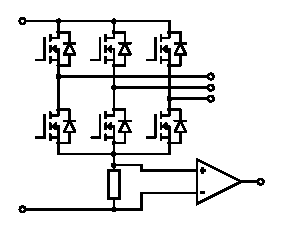
\includegraphics[width=0.5\columnwidth]{Slike/Inkscape/inverter.eps}
    \caption{\label{inverter} Shema močnostnega pretvornika in meritve toka }
\end{figure}

Na sliki \ref{inverter} je prikazan močnostni pretvornik, prav tako pa je prikazano merjenje toka. Uporabljena je konfiguracija enega shunta, kar pomeni, da ko bodo vse tri faze na napajalni
napetosti ali na 0V, skozi shunt ne bo tekel tok. Zato meritev delamo na začetku PWM periode, ko naprej preklopimo prvo fazo, nato pa drugo. Na sliki \ref{meritevTokaIu} je prikazana prva meritev.
Če definiramo tok, ki teče v stroj kot pozitiven tok, v tem času merimo tok $i_u$, saj teče iz prve faze v stroj, se porazdeli med drugo in tretjo fazo in skozi shunt. 

\begin{figure}[!htbp]
    \centering
    \includegraphics[width=0.5\columnwidth]{Slike/Inkscape/meritevTokaIu.eps}
    \caption{\label{meritevTokaIu} Meritev toka $i_u$ }
\end{figure}

Na sliki \ref{meritevTokaIw} pa je prikazana druga meritev, kjer tok steče skozi prvo in drugo fazo v stroj, iz tretje faze stroja pa skozi shunt, zato tukaj merimo negativen tok $i_w$. 

\begin{figure}[!htbp]
    \centering
    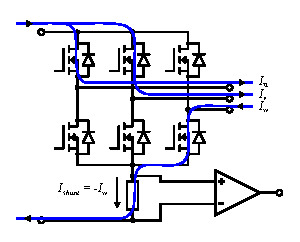
\includegraphics[width=0.5\columnwidth]{Slike/Inkscape/meritevTokaIw.eps}
    \caption{\label{meritevTokaIw} Meritev toka $-i_w$ }
\end{figure}

Tok druge faze $i_v$ pa izračunamo po enačbi \ref{izracunIv} iz dveh meritev, saj velja $i_u + i_v + i_w = 0$.

\begin{equation} \label{izracunIv}
i_v = -(i_u + i_w)
\end{equation}

Na sliki \ref{fazeInShunt} so prikazane vse tri fazne napetosti in izhod ojačevalnika. Prvi dve svetlo sivi območji označujeta merilno okno tokov $I_u$ in $- I_w$, v tretjem oknu pa merimo napetost
izhoda ojačevalnika pri toku 0 A. Za meritev dejanskega toka moramo od meritve prvega in drugega okna odšteti meritev tretjega.

\begin{figure}[!htbp]
    \centering
    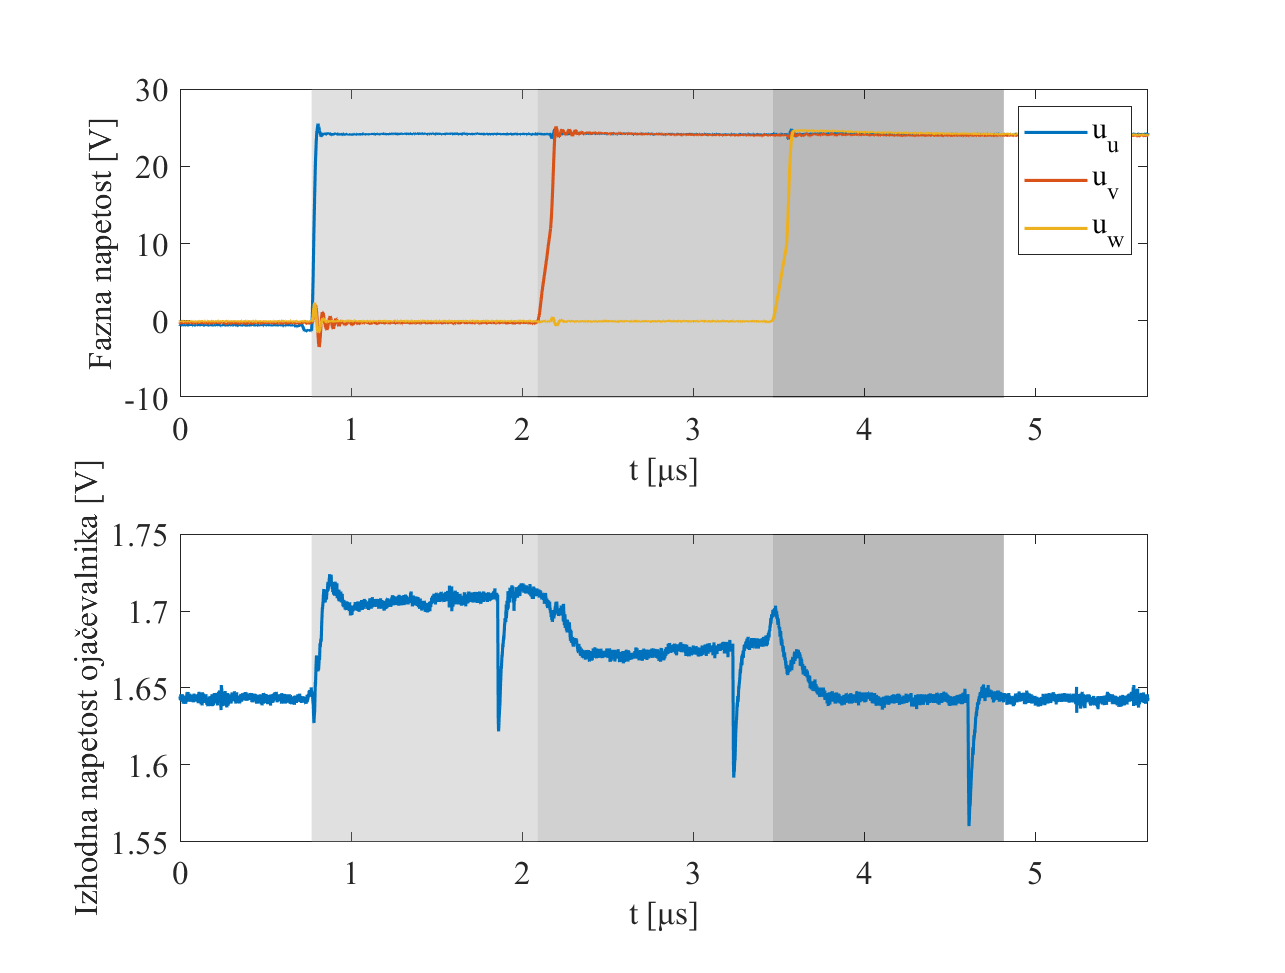
\includegraphics[width=1\columnwidth]{Slike/fazeInShunt.eps}
    \caption{\label{fazeInShunt} Fazne napetosti in ojačan signal shunta. }
\end{figure}

%*******************************************************************************
%**                             Rezultati                         
%*******************************************************************************
\newpage
\section{Rezultati} \label{rezultati}

V času razvoja algoritma je bilo opaženo, da se ta odziva drugače pri različnih pogojih. Prvi način obratovanja je, ko rotor hitro pospeši do končne hitrosti brez povečanega bremenskega navora. Drugi
način pa je obratovanje s povečanim bremenskim navorom oziroma, ko se rotor vrti počasi. 

Na sliki \ref{NoLoadRun} je prikazano delovanje algoritma in ocena pozicije brez dodatnega bremenskega navora. Napaka ocene je relativno majhna, vendar se na toku $I_e$ opazi
višjeharmonsko popačenje. Ker je vrtilna hitrost visoka, regulator toka $I_e$ ni zmožen odpraviti popačenja, zato popačenje ne vpliva na oceno pozicije rotorja.

\begin{figure}[!htbp]
    \centering
    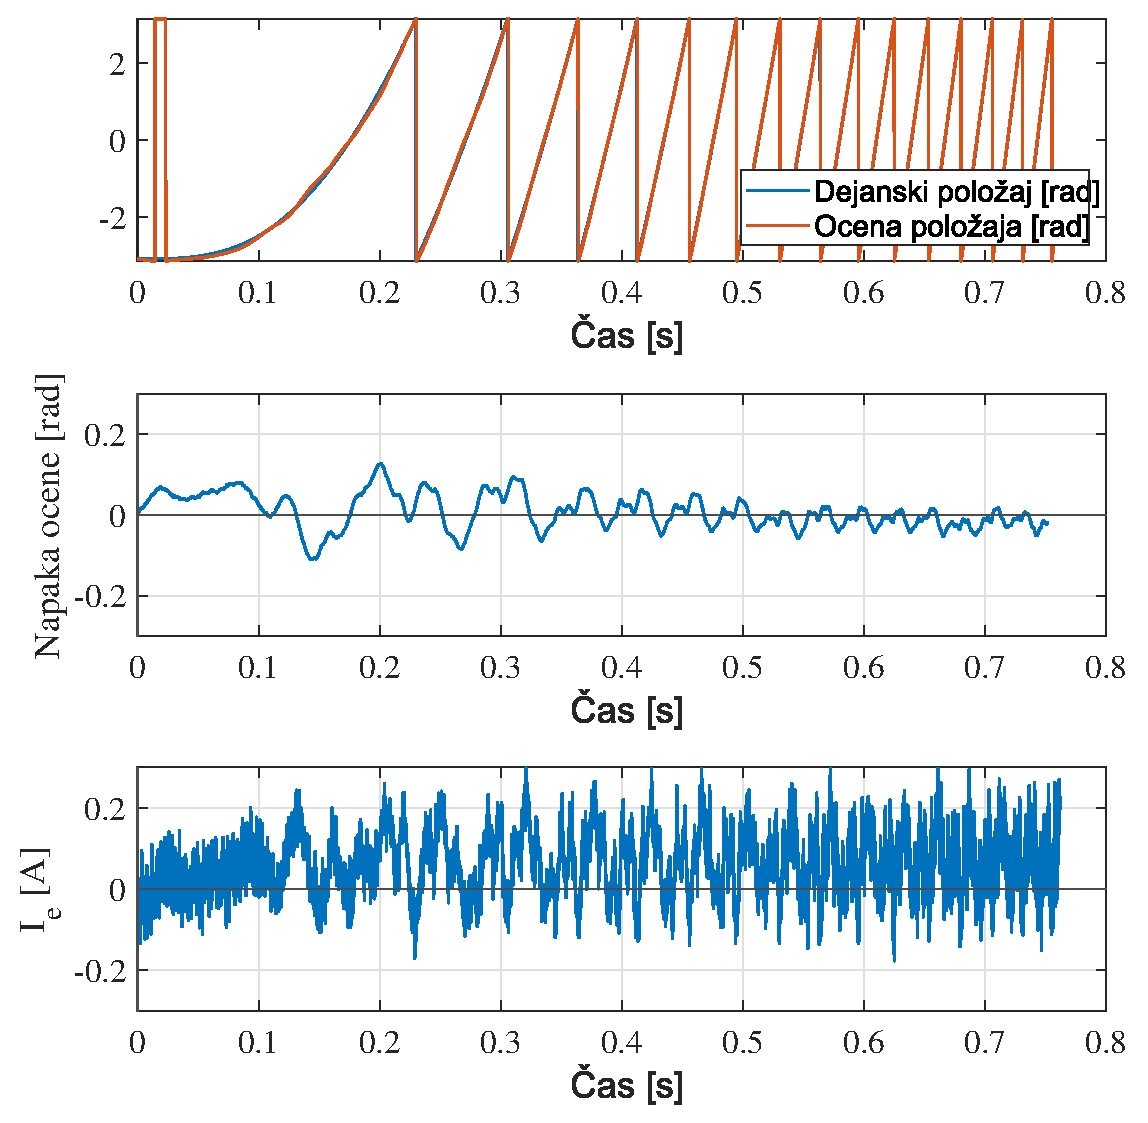
\includegraphics[width=0.9\columnwidth]{Slike/NoLoadRun.eps}
    \caption{\label{NoLoadRun} Ocena pozicije rotorja in tok $I_e$ pri obratovanju brez dodatnega bremena. }
\end{figure}

\newpage

Na sliki \ref{HighLoadRun} pa smo rotor vrteli s hitrostjo približno enega obrata na 10 sekund. Ko se stroj vrti z nizko hitrostjo, pa regulator toka odpravi višjeharmonsko popačenje kot se opazi na
tretjem grafu. Vendar pa to vpliva na oceno pozicije, saj z regulacijo napake (npr. visokoharmonsko popačenje) v toku $I_e$, nastane napaka na oceni pozicije.

\begin{figure}[!htbp]
    \centering
    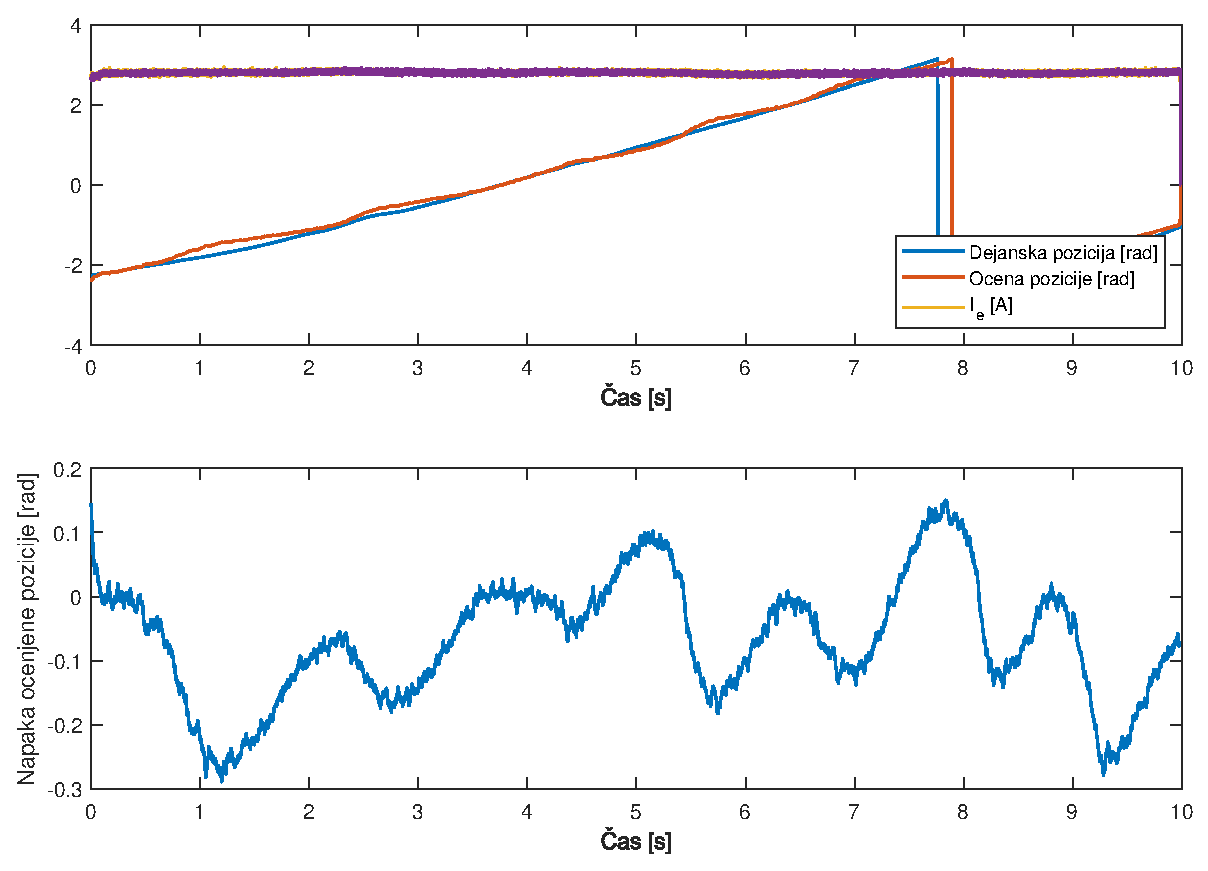
\includegraphics[width=0.9\columnwidth]{Slike/HighLoadRun.eps}
    \caption{\label{HighLoadRun} Ocena pozicije rotorja in tok $I_e$ pri nizki vrtilni hitrosti. }
\end{figure}

\newpage 

Višjeharmonsko popačenje je odvisno od enosmerne komponente prečnega toka. To se opazi tudi na oceni kota, kot je prikazano na sliki \ref{vsiljenaPozicijaTokovi_angleError}. Opazimo, da je napaka
ocene pozicije rotorja pri nižjih prečnih tokovih majhna in relativno nespremenljiva, z višjimi tokovih pa postane večja. Na napaki ocenjene pozicije se lahko direktno opazi efekt višjeharmonskega
popačenja. 

\begin{figure}[!htbp]
    \centering
    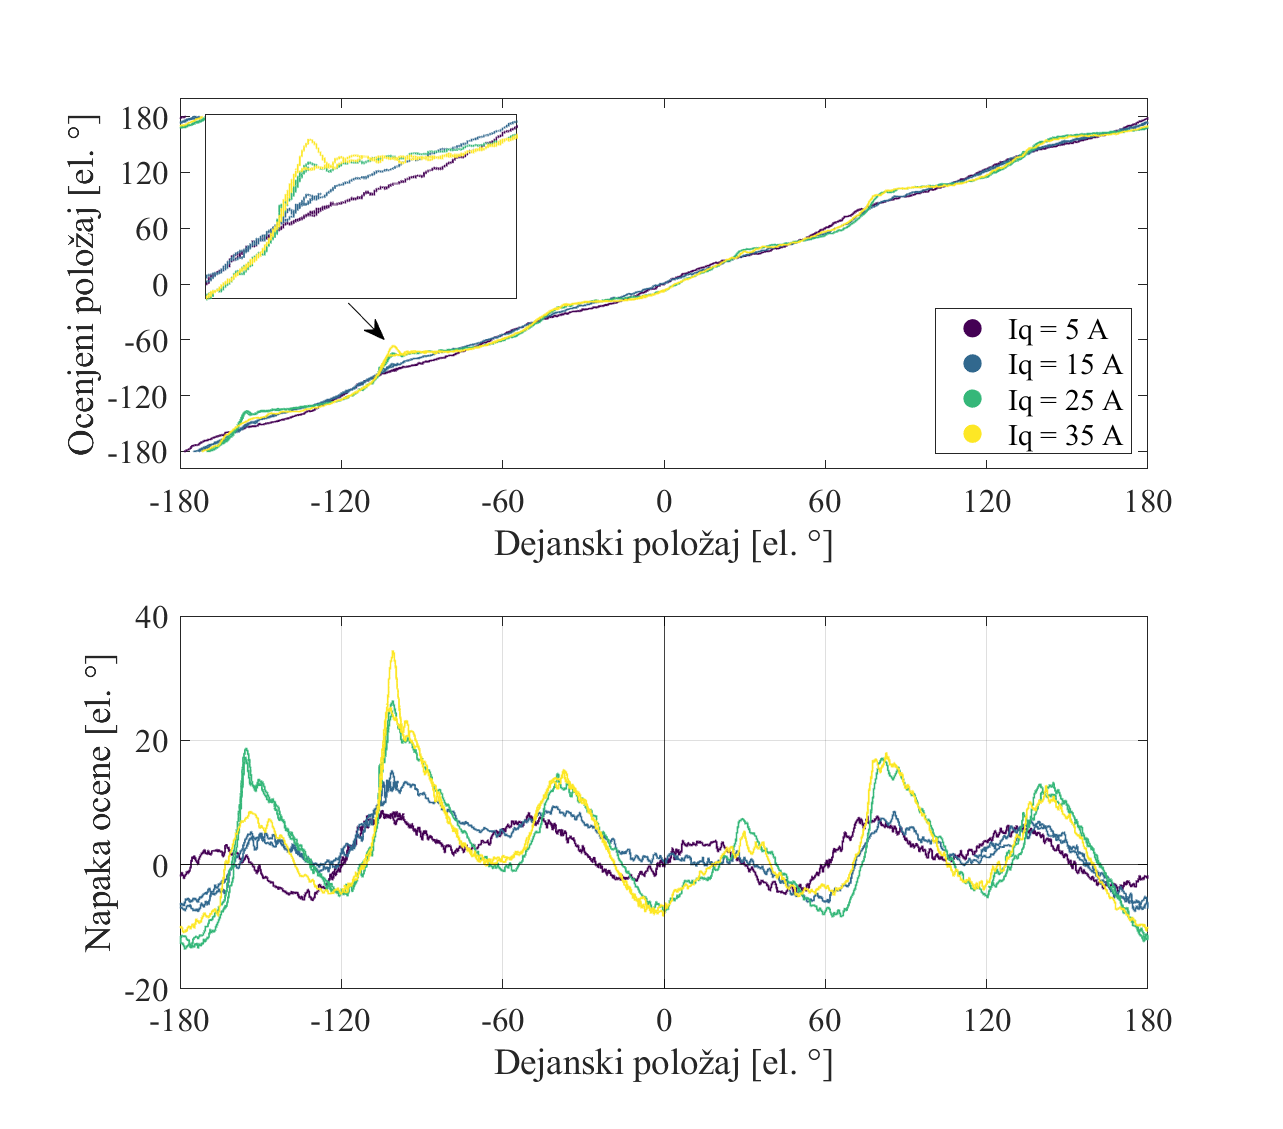
\includegraphics[width=1.05\columnwidth]{Slike/vsiljenaPozicijaTokovi_angleError.eps}
    \caption{\label{vsiljenaPozicijaTokovi_angleError} Ocena pozicije rotorja in napaka ocene pri različnimi prečnimi tokovi. }
\end{figure}

Poglejmo še vpliv mrtvega časa - pokazali smo, da ima ta vpliv na tok $I_e$, ki je v času efekta mrtvega časa močno popačen. Na sliki \ref{vsiljenaPozicijaMrtviCasPlot_angleError} je prikazan vpliv
mrtvega časa na oceno pozicije, kjer je bila enosmerna komponenta prečnega toka 20 A. Vidimo, da je na pozicijah $k\frac{\pi}{3}$ prisotna napaka ocene. To je ravno takrat, ko s faznimi tokovi
preidemo čez nič.

\begin{figure}[!htbp]
    \centering
    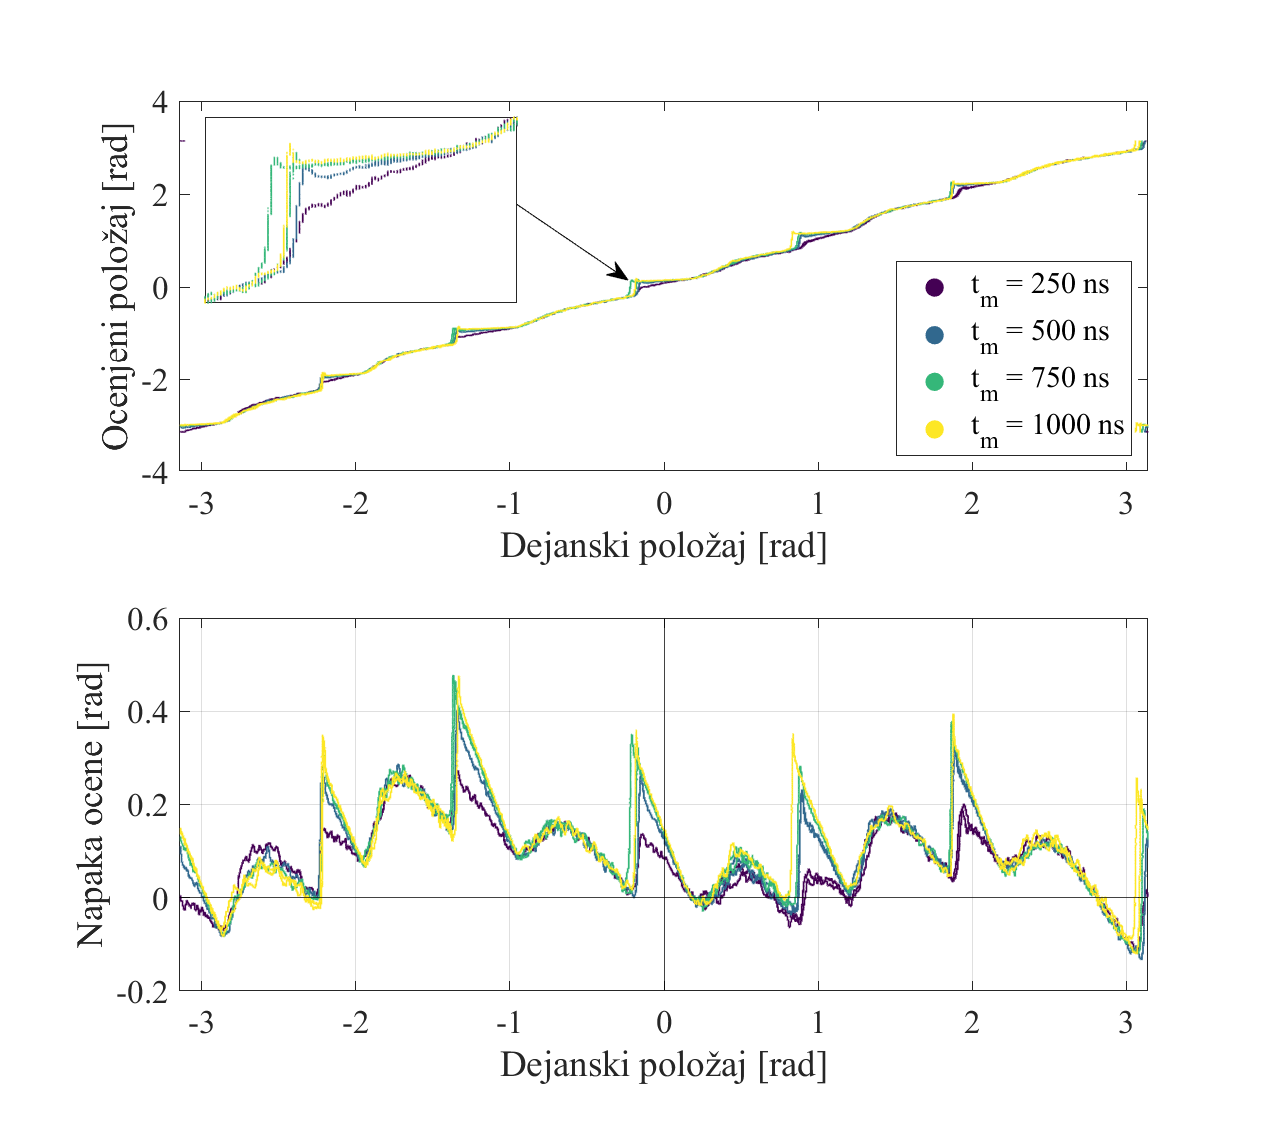
\includegraphics[width=1.05\columnwidth]{Slike/vsiljenaPozicijaMrtviCasPlot_angleError.eps}
    \caption{\label{vsiljenaPozicijaMrtviCasPlot_angleError} Ocena pozicije rotorja in napaka ocene pri različnimi vrednostmi mrtvega časa. }
\end{figure}

\newpage

Na sliki \ref{vsiljenaPozicijaMrtviCasPlot_angleError} je prikazan eksperiment, kjer je bil mrtvi čas 1 μs, spreminjala pa se je enosmerna komponenta prečnega toka. Pri nižjih prečnih tokovih
prevladuje efekt mrtvega časa, pri višjih pa efekt višjeharmonskega popačenja.

\begin{figure}[!htbp]
    \centering
    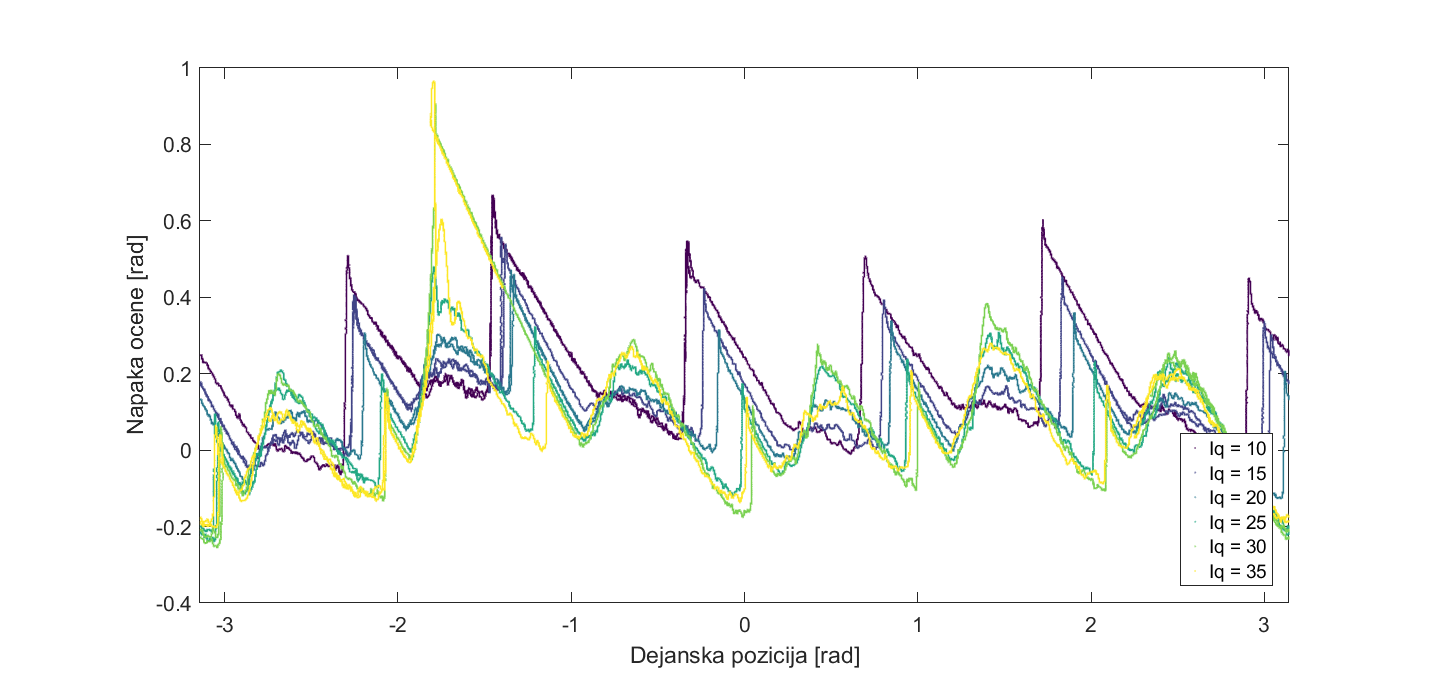
\includegraphics[width=1.05\columnwidth]{Slike/vsiljenaPozicijaTokoviZMrtvimCasom_angleError.eps}
    \caption{\label{vsiljenaPozicijaTokoviZMrtvimCasom_angleError} Napaka ocene kota pri različnimi prečnimi tokovi in velikim mrtvim časom. }
\end{figure}

Pri tem eksperimentu je bil mrtvi čas 1 μs, kar je relativno velika vrednost. V praksi je mrtvi čas precej nižji, ne moremo pa se mu izogniti, zato je bil prikazan njegov vpliv.

%================================================================================
%================================================================================
%**                             Zaključek                           
%================================================================================
%================================================================================
\chapter{Zaključek} \label{zakljucek}

V sklopu te magistrske neloge smo izdelali algoritem za ocenjevanje pozicije rotorja pri nizkih hitrostih in v nevrtečem stanju. Najprej smo matematično izpeljali pričakovani tokovni odziv kot
posledica vzbujanja in rotorske pozicije. Nato smo pokazali vzbujanje na realnem sistemu in kako ta odstopa od pričakovanega. Dodatno smo pokazali kako mrtvi čas vpliva na tokovni odziv. Opazili smo,
da oceno pozicije najbolj kvari višjeharmonsko popačenje v d-q HKS, katerega nam ni uspelo pojasniti in razrešiti. 

Pokazali smo tudi vpliv enosmernega prečnega toka na delovanje algoritma in opazili, da z višjimi tokovi algoritem deluje slabše, ker se višjeharmonsko popačenje poveča. Pri nižjih tokovih pa se
poveča vpliv mrtvega časa, kar pa lahko mitigiramo z nižanjem le-tega ali nižanjem amplitude vzbujalnega signala.

V primeru nadaljnih raziskav bi bilo smiselno raziskati vir višjeharmonskih popačenj in možne kompenzacije.

%******************************* LITERATURA ************************************
\cleardoublepage\phantomsection\addcontentsline{toc}{chapter}{Literatura} % vnos literature v kazalo

% 1. način: BibTeX
\bibliographystyle{ieeetrslo}
\bibliography{literatura}

% 2. način: neposreden vnos \begin{thebibliography}{99} \bibitem{vir1} C. Su, H. Ke in T. Hubing, ``Overview of Electromagnetic Modeling Software'' [Online], v \textit{25th Annual Review of Progress
%    in Applied Computational Electromagnetics, March 8 - March 12, 2009 - Monterey, California}. Monterey, 2009, str. 736-741. Dosegljivo: \url{http://www.clemson.edu/ces/cvel/pdf/ACES09-736.pdf}.
%    [Dostopano: 23.8.2017]. \bibitem{vir2} T. Hubing et al., ``Survey of Current Computational Electromagnetics Techniques and Software'' [Online]. \textit{Clemson University Vehicular Electronics
%    Laboratory (CVEL)}: Clemson, ZDA, CVEL-08-011.2, 21.9.2008. Dosegljivo: \url{http://www.clemson.edu/ces/cvel/Reports/CVEL-08-011.2.pdf}. [Dostopano: 23.8.2017]. \bibitem{vir3} \textit{The
%    Electromagnetic Radiation Spectrum Poster} [Online]. Dosegljivo: \url{http://www.unihedron.com/projects/spectrum/}. [Dostopano: 23.8.2017]. \end{thebibliography}

%******************************* DODATEK ***************************************
\appendix

Na slikah \ref{PItuning_Kp_unstableLow} - \ref{PItuning_Kp_stable} so prikazani vplivi različnih vrednostih $K_p$ na oceno pozicije rotorja, slike \ref{PItuning_Ki_unstableLow} -
\ref{PItuning_Ki_stable} pa prikazujejo vpliv $K_i$ parametra.

\begin{figure}[!htbp]
    \centering
    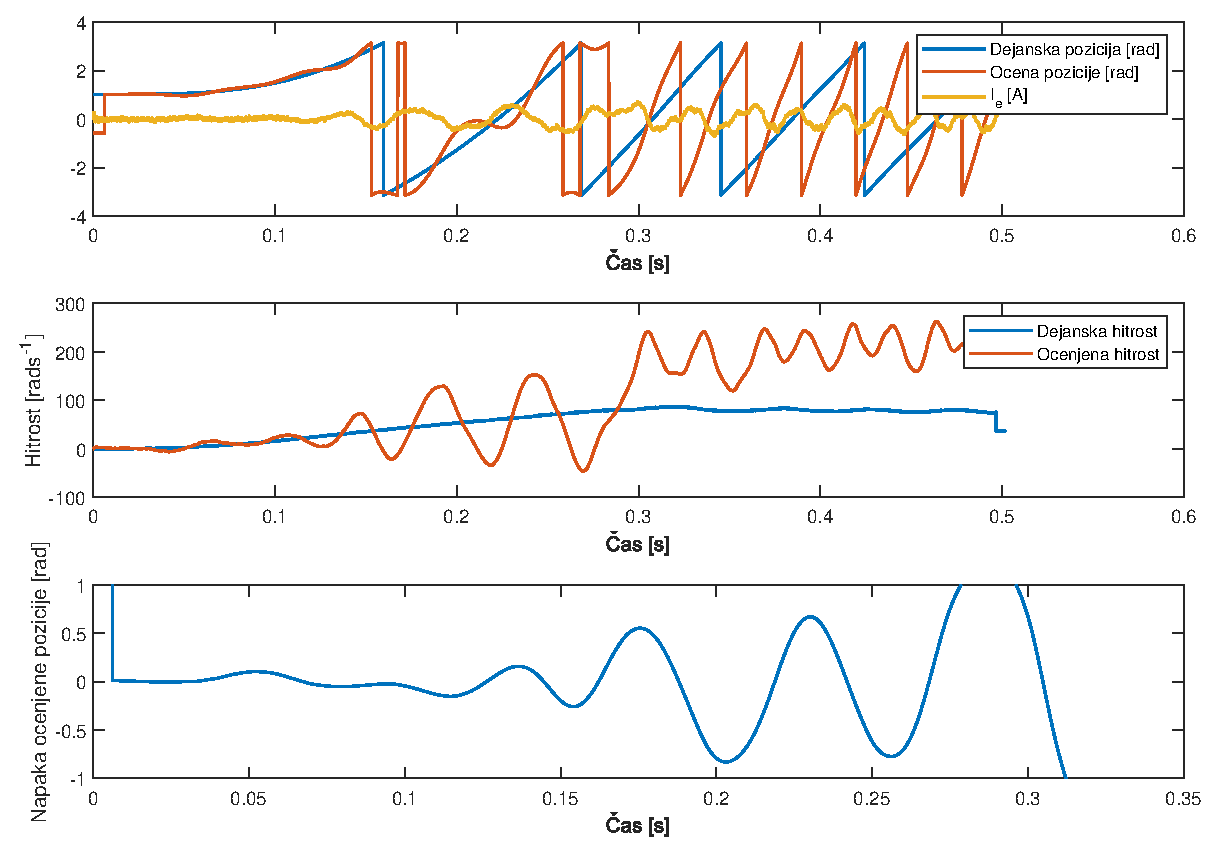
\includegraphics[width=1\columnwidth]{Slike/PItuning_Kp_unstableLow.eps}
    \caption{\label{PItuning_Kp_unstableLow} Prikaz vpliva premajhnega $K_p$ parametra. }
\end{figure}

\begin{figure}[!htbp]
    \centering
    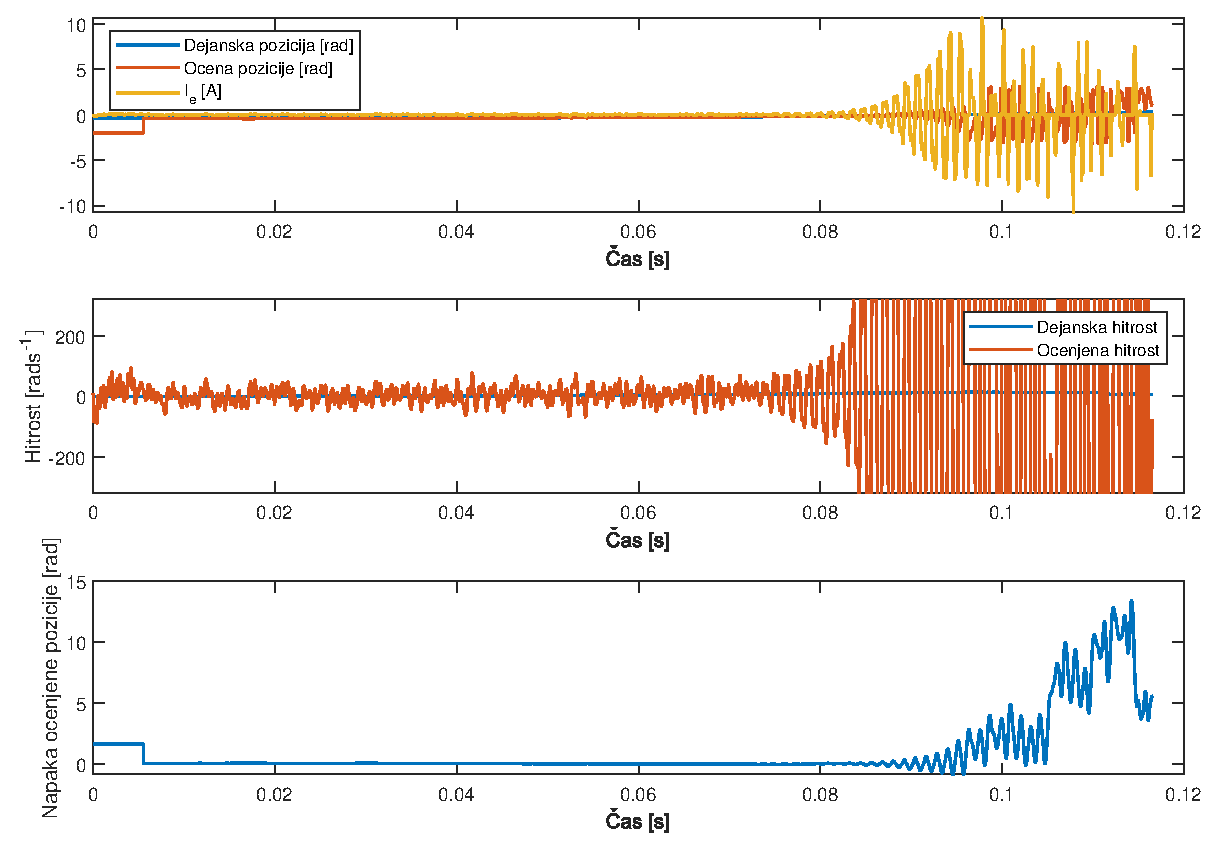
\includegraphics[width=1\columnwidth]{Slike/PItuning_Kp_unstableHigh.eps}
    \caption{\label{PItuning_Kp_unstableHigh} Prikaz vpliva prevelikega $K_p$ parametra. }
\end{figure}

\begin{figure}[!htbp]
    \centering
    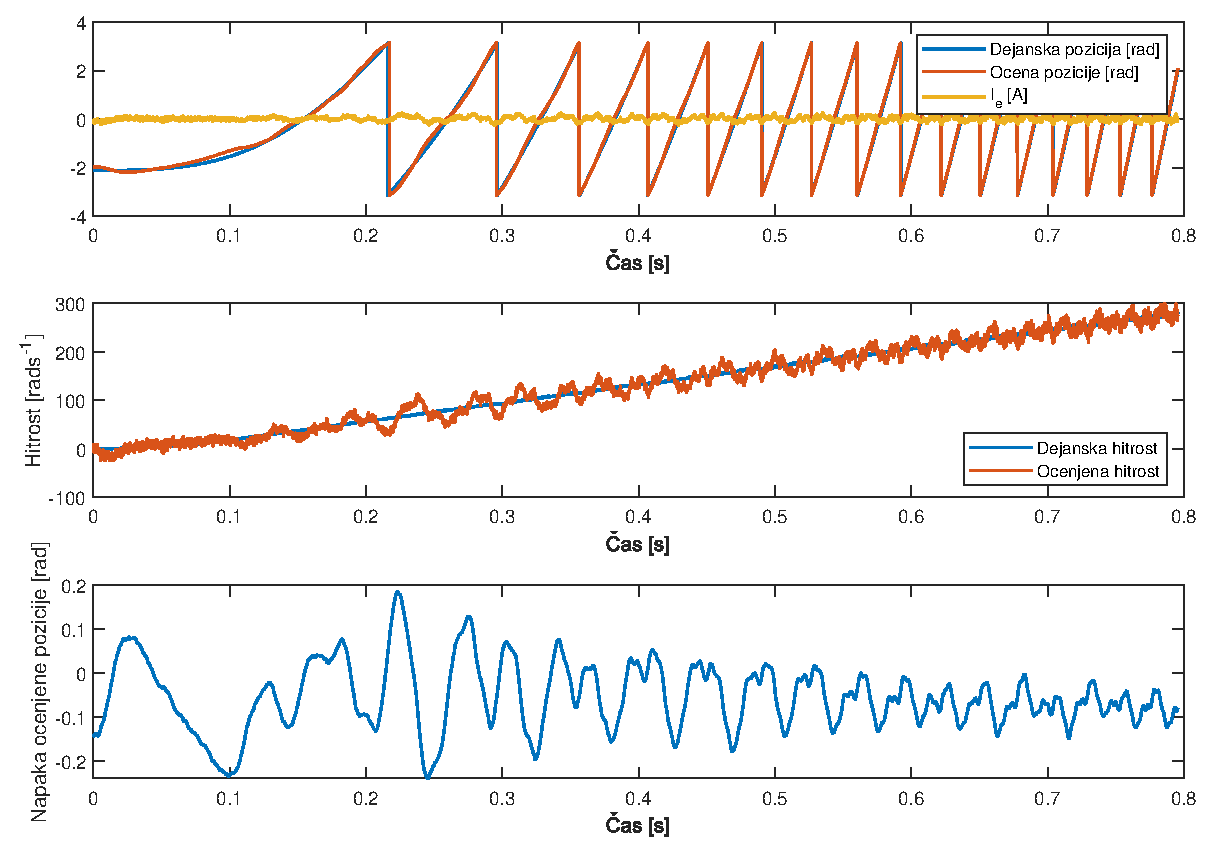
\includegraphics[width=1\columnwidth]{Slike/PItuning_Kp_stable.eps}
    \caption{\label{PItuning_Kp_stable} Prikaz vpliva optimalnega $K_p$ parametra. }
\end{figure}

\begin{figure}[!htbp]
    \centering
    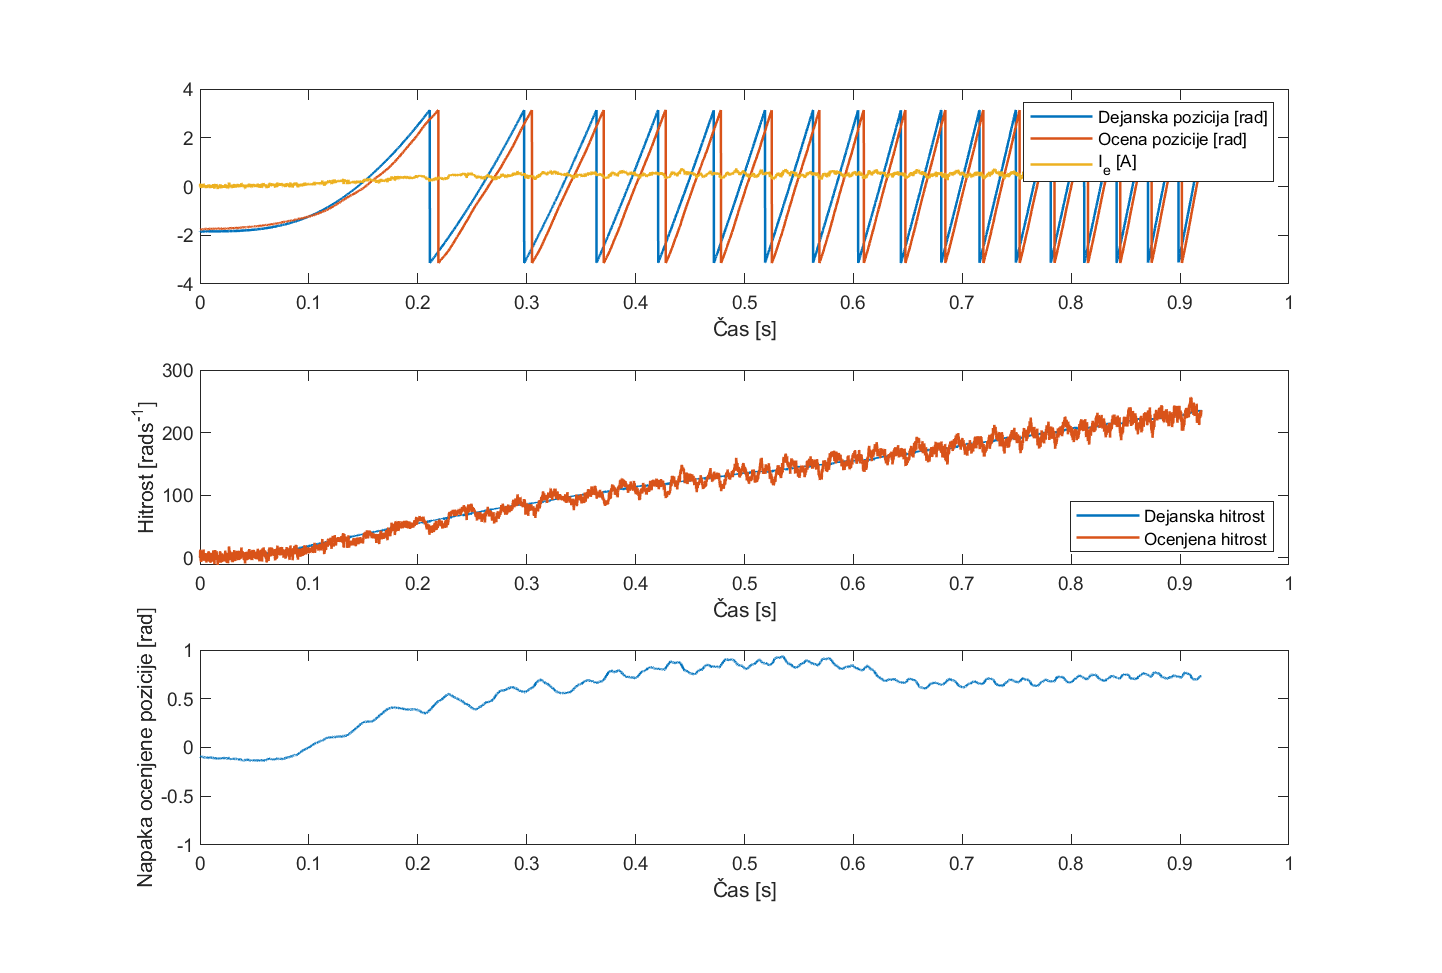
\includegraphics[width=1\columnwidth]{Slike/PItuning_Ki_unstableLow.eps}
    \caption{\label{PItuning_Ki_unstableLow} Prikaz vpliva premajhnega $K_i$ parametra. }
\end{figure}

\begin{figure}[!htbp]
    \centering
    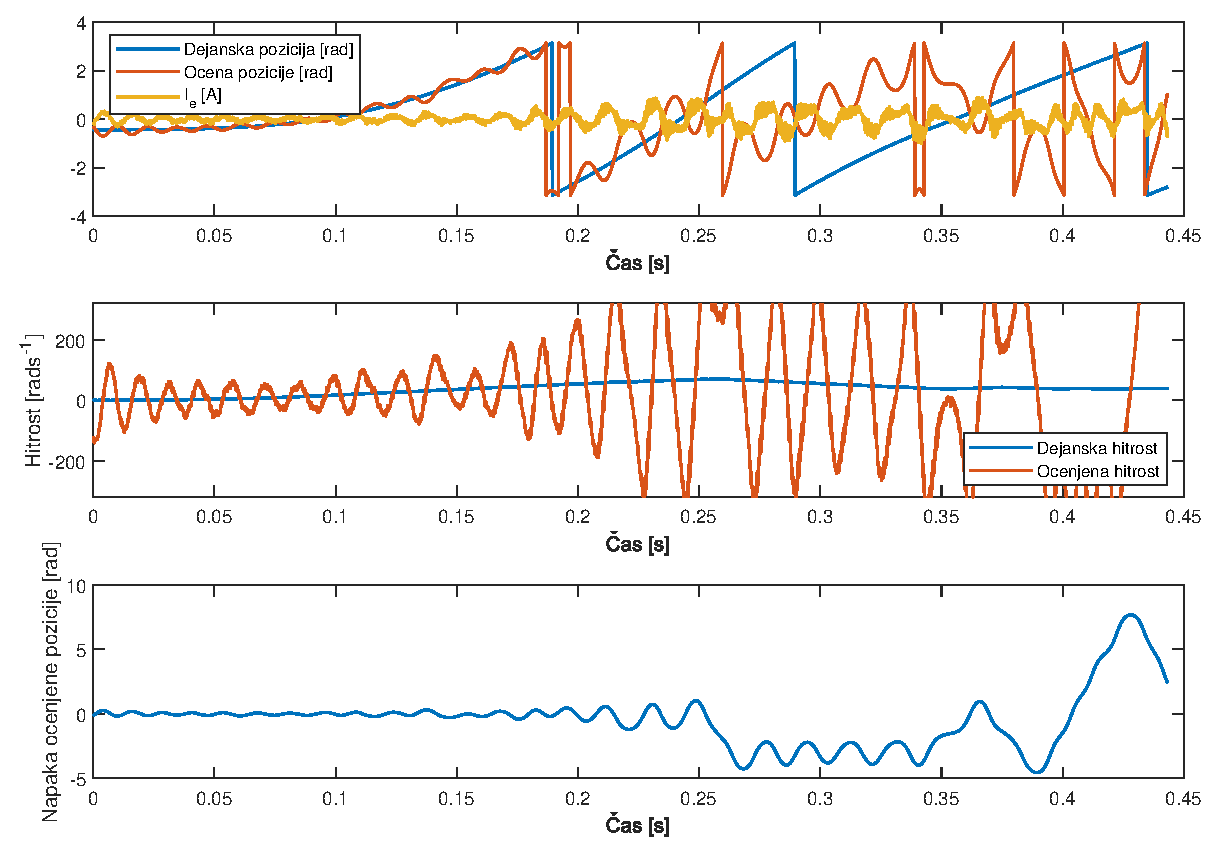
\includegraphics[width=1\columnwidth]{Slike/PItuning_Ki_unstableHigh.eps}
    \caption{\label{PItuning_Ki_unstableHigh} Prikaz vpliva prevelikega $K_i$ parametra. }
\end{figure}

\begin{figure}[!htbp]
    \centering
    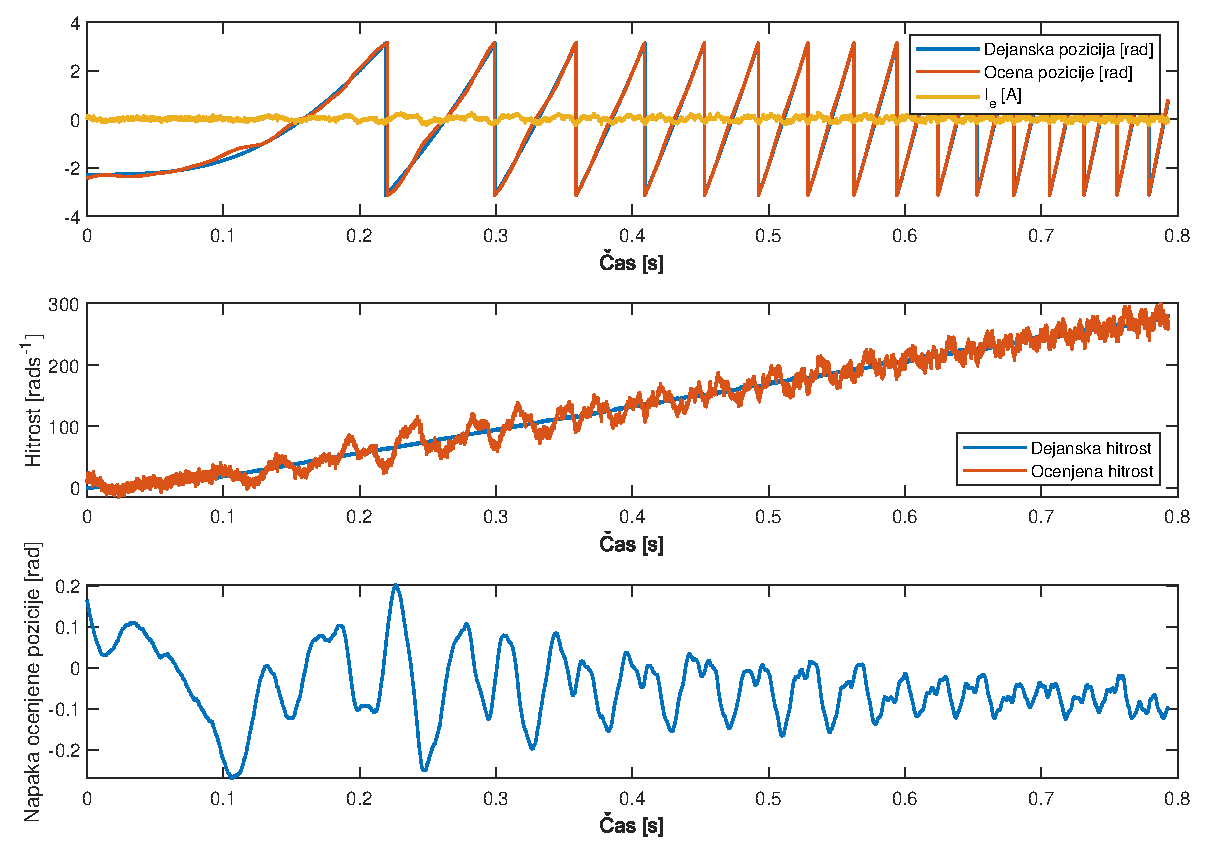
\includegraphics[width=1\columnwidth]{Slike/PItuning_Ki_stable.eps}
    \caption{\label{PItuning_Ki_stable} Prikaz vpliva optimalnega $K_i$ parametra. }
\end{figure}

\end{document}
%%%%%%%%%%%%%%%%%%%%%%%%%%%%%%%%%%%%%%%%%%%%%%%%%%%%%%%%%%%%%%%%%%%%%%%%%%%%%%%%%%%%%%%%%%%%%%%%%%%%%%%%%%%%%%%%%%%%%%%%
